\documentclass[titlepage, a4paper, 11pt]{scrartcl}

%too much whitespace otherwise
\usepackage[left=2cm,right=2cm,top=2cm,bottom=2cm]{geometry}

% Grafik Pakete
\usepackage{graphicx,hyperref,amssymb}

% Ordner für Grafiken
\graphicspath{ {./Grafiken/} }
\usepackage{float}

\usepackage[utf8]{inputenc}
\usepackage[german]{babel}
\usepackage[T1]{fontenc}
\usepackage{amsmath}
\usepackage{amsfonts}
\usepackage{amssymb}
\usepackage{graphicx}

\usepackage{caption}
\usepackage{subcaption}

% Header and Footer
\usepackage{fancyhdr}

%bibtex
\usepackage{cite}

%code snippets
\usepackage{listings}
\usepackage{color}

\definecolor{dkgreen}{rgb}{0,0.6,0}
\definecolor{gray}{rgb}{0.5,0.5,0.5}
\definecolor{mauve}{rgb}{0.58,0,0.82}

\lstset{frame=tb,
  language=HTML,
  aboveskip=3mm,
  belowskip=3mm,
  showstringspaces=false,
  columns=flexible,
  basicstyle={\small\ttfamily},
  numbers=none,
  numberstyle=\tiny\color{gray},
  keywordstyle=\color{blue},
  commentstyle=\color{dkgreen},
  stringstyle=\color{mauve},
  breaklines=true,
  breakatwhitespace=true,
  tabsize=3
}


\pagestyle{fancy}
\fancyhf{}
\rhead{Lückert, Neudecker, Schnoor}
\lhead{AR Exhibition - Dokumentation}

\title{AR Exhibition - A LiDAR powered AR Application}
\author{Marlon Lückert \\ Bachelor of Science \\ \href{mailto:marlon.lueckert@haw-hamburg.de}{marlon.lueckert@haw-hamburg.de} 
\and Julius Neudecker \\ Bachelor of Science \\ \href{mailto:julius.neudecker@haw-hamburg.de}{julius.neudecker@haw-hamburg.de}
\and Vincent Schnoor \\ Bachelor of Science \\ \href{mailto:vincent.schnoor@haw-hamburg.de}{vincent.schnoor@haw-hamburg.de} }
\date{November 2020}


\begin{document}

  \maketitle

  \tableofcontents

  \begin{abstract}
    Diese Dokumentation befasst sich mit der Entwicklung und den Hintergründen der ARExhibition App, welche ein Teil des XRchitecture-Projekts ist.
    Wir geben vorab eine Gesamtübersicht über alle Teilaspekte des Projekts und schaffen den Kontext zum Gesamtprojekt.S
    Im zweiten Teil gehen wir auf die Details der Umsetzung ein, die sich in zwei Teile gliedern: die Client App auf dem mobilen Endegerät und das Backend zum Speichern der Daten.
    Der letzte Teil befasst sich mit der Evaluation der Anwendung und der Frage, ob durch die neue LiDAR-Technologie ein Mehrwehrt in der User-Experience generiert werden kann.
  \end{abstract}

  \section{Projektbeschreibung}
    % Wovon handelt das Projekt? Wie ist es entstanden? Warum ist es interessant?
    Das Projekt \textit{ARExhibition}, welches im Rahmen des Projektes \textit{XRchitecture} entstanden ist macht das Ausstellen digitaler Modelle und Medien einfacher. 
    Mit nur wenigen Klicks können 3D-Modelle, Bilder und Videos aus einem hierfür entwickelten Content-Management-System (CMS) in AR platziert und gespeichert werden. 
    Die so entstandenen AR-Szenen können von Besuchern über einen Marker geladen und betrachtet werden.\\
    Diese Ausstellungen können bspw. von Hochschulen und anderen Bildungsinstituten genutzt werden um Projekte der Studierenden und Schüler auszustellen.

    \subsection{Projektziel}
      % Was soll erreicht werden?
      Das erste Ziel des Projektes ist es, eine Plattform für die Studierenden der HAW zu schaffen, um ihre im Semester erstellten 3D-Modelle, 
      Bilder und Videos an einem zentralen Ort zu speichern und mit anderen Studierenden zu teilen.

      Das zweite Ziel des Projektes ist es eine Augmented Reality App zu entwickeln, welche es ermöglicht besagte mediale Inhalte in einem Raum zu platzieren und jederzeit dort wieder abrufbar zu machen.
      Dabei soll die Position der Inhalte für jeden Nutzer exakt die Gleiche sein, wodurch die soziale Interaktion zwischen Usern angetrieben werden soll.
      Die AR App soll ohne einen großen organisatorischen Aufwand für alle Nutzergruppen zu bedienen sein, das heißt, dass das Tracking möglichst ohne externe Maker und Aufbauten auskommen muss.

    \subsection{Zielgruppen}
      % Welche Zielgruppen werden mit dem Produkt angesprochen und warum?
      Für unser aus zwei Teilen bestehendes Projekt gibt es zwei Zielgruppen.\\
      Die erste Zielgruppe besteht aus den Studenten der HAW welche das Content-Management-System zum einfachen Teilen ihrer Arbeiten nutzen können. 
      Die Projekte anderer Studiengänge und Fakultäten können so leichter eingesehen werden. Außerdem können die Arbeiten anderer Studenten heruntergeladen und für eigene Studienprojekte verwendet werden.\\

      Bildungsinstitute wie die HAW Hamburg und Bildungsstätten wie Museen bilden die zweite Zielgruppe. 
      Für bspw. die HAW Hamburg wird die Ausrichtung von Ausstellungen der Studentenprojekte vereinfacht, da Räume interaktiver und sinnvoller mit digitalen Medien gefüllt werden können. 
      Wo vorher 3D-Objekte auf PC Bildschirmen betrachtet werden mussten, können diese mithilfe der App als Teil des Raumes betrachtet und mit ihnen interagiert werden. 
      Museen und Ausstellungen können durch die App ihr Repertoire an Kunst und Objekten erweitern, da virtuelle Bilder und Objekte einfach ausgestellt werden können. 
      Die Inhalte können genau wie vom Kurator gewollt platziert werden und erscheinen dem Besucher in der gewollten Position, Rotation und Größe.

  \section{Technische Umsetzung}
  % Wie funktioniert die App, bzw. das CMS? Welche Software/Hardware Einheiten werden verwendet?
  Das Projekt besteht im Wesentlichen aus zwei Komponenten: 
  ein Content-Management-System, welches die Bereitstellung und Verwaltung der Inhalte und Szenen übernimmt - im Folgenden \textit{CMS} genannt -
  und einer App auf einem mobilen Endgerät, welche die Platzierung virtueller Inhalte in einem Raum in AR ermöglicht - nachfolgend als \textit{App} bezeichnet.\\

  In diesem Kapitel werden zunächst die Details zum Aufbau und zur Implementierung des CMS und der App erläutert.
  Ferner gehen wir auf ähnliche, bereits existierende Produkte ein und inwieweit sich unser Produkt von diesen abgrenzt.
  Dabei gehen wir ann entsprechender Stelle auch auf ganz bewusste Designentscheidungen ein und warum wir an einigen Stellen Abwägungen treffen mussten.
  
  \begin{figure}[h]
    \centering
    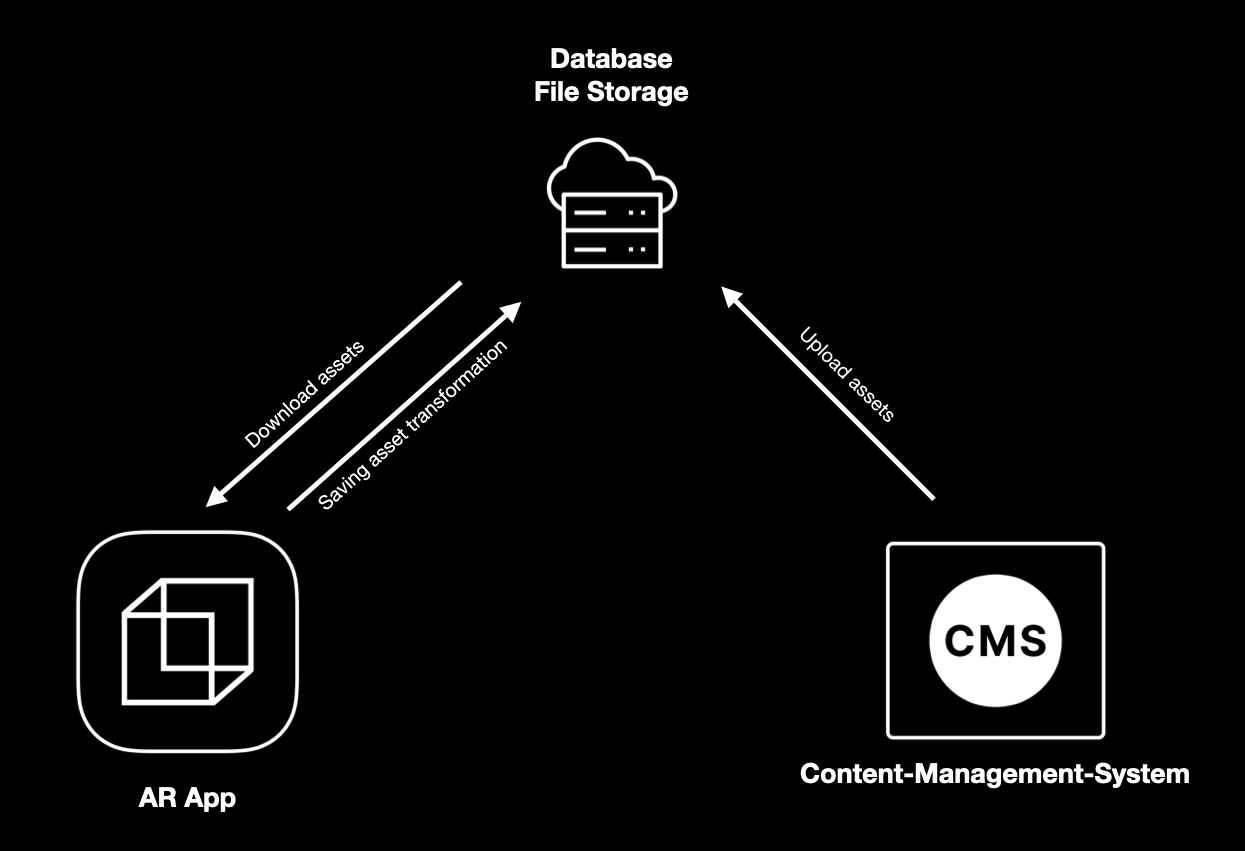
\includegraphics[width=.6\textwidth]{project-structure}
    \caption{Projekt Struktur}
    \label{ProjektStruktur}
  \end{figure}

  In Abbildung \ref{ProjektStruktur} ist der Zusammenhang zwischen den Projektteilen skizziert.
  Auf der einen Seite ist das Content-Management-System zu finden, welches über eine Weboberfläche das Hochladen von Assets ermöglicht.
  Die hochgeladenen Dateien werden auf dem File Server gespeichert und es werden Datenbankeinträge für die Asset Informationen angelegt.
  Die AR App konsumiert die Assets des File Servers, welche vom Kurator platziert werden. Die Einrichtung des Kurators wird persistent in der Datenbank gespeichert. 
  
  Durch das Entkoppeln von Daten und Anwendunglogik ist es möglich die Downloadgröße der App auf ein Minimum zu reduzieren.
  Außerdem können die Daten der App zu jedem Zeitpunkt erweitert oder ausgetauscht werden ohne eine neue Version der App zu veröffentlichen. 

  Diese Struktur ermöglicht es auch weitere Services einzubinden, die entweder die Assets der Datenbank nutzen oder Assets für die App bereitstellen.
  Die VR-Applikation \textit{XRchitecture} ist ein Beispiel für eine Anwendung, die die hochgeladenen Assets einbinden könnte.
  Als weiterer Asset Lieferant könnten beispielsweise Plattformen wie \textit{Sketchfab} eingesetzt werden. 

    \subsection{Stand der Forschung}
    % Welche Literatur liegt dem Projekt zugrunde, bzw. welche anderen Produkte/Projekte? Inwiefern grenzt sich unser Projekt von diesen ab?

      Weil die Technologie der Augemented Reality schon seit einiger Zeit existiert, haben sich bereits Forscher und kommerzielle Vorhaben dieser Thematik gewidmet,
      um die Anwendung von AR auch in Ausstellungskontexten zu untersuchen.

      Eins der älteren Paper ist von Narumi et. al.\cite{narumi2011digital}, die mittels AR Dioramen mit virtuellen Content überlagert haben.
      Entgegen unserem Ansatz findet das allerdings als Projektionsüberlagerung statt.

      Okada et. al. haben Mobile Devies genutzt, um Bilder vergangener Tage im Rahmen einer Ausstellung im öffentlichen Raum auf Oberflächen darzustellen\cite{okada2015manseibashi}.
      Weil das Projekt bereits vor 5 Jahren umgesetzt wurde, konnte hier noch keine LiDaR Technologie eingesetzt werden. 
      Auch wurde hier die soziale Akzeptanz einer solchen Ausstellung untersucht. Wir haben andere Schwerpunkte gesetzt.

      Fuguo und Jing haben 2017 untersucht, wie man Ausstellungen mithilfe des Vuforia AR-Frameworks mit digitalen Inhalten anreichern kann\cite{peng2017mobile}. Durch große Fortschritte
      im Bereich der Tracking Technologien wird ein Tracking des realen Raumes durch Bildmarker - wie im damaligen Vuforia Framework - obsolet.

      Es ist allgemein zu beobachten, dass sich im Zeitraum 2015-2018 zahllose Forschungsarbeiten mit der Technologie der Augmented Reality auseinandergesetzt haben,
      um deren Einsatz im Ausstellungskontext zu untersuchen. Bei diesen Arbeiten liegt der Fokus mehr auf der Untersuchung des Mediums als solches. Wir grenzen uns insofern ab,
      als das bei uns der Content im Vordergrund steht. Wie kann man Content zentral speichern und verwalten und wie man für mehrere Nutzer ein konsistentes Erlebnis 
      erreichen kann.

      \pagebreak

    \subsection{Content-Management-System}

      Unser CMS ist einerseits Kombination aus einem Frontend für bspw. Upload von Content, Betrachten des zur Verfügung stehenden Contents und Pflege von Szenen und Metadaten 
      und andererseits einem Backend, was die Daten im Hintergrund speichert, verwaltet und auf Abfrage zur Verfügung stellt. Je nach Umfang und Struktur des Projekts spricht man ggfs. auch 
      von der sog. \textit{Middleware}. Dieser Begriff ist häufig sehr abstrakt definiert und wobei die Grenze zwischen Frontend und Middleware recht eindeutig ist,
      ist sie zwischen Middleware und Backend sehr viel schwieriger zu ziehen. In unserem Fall ist die Middleware zum Zwecke der Einfachheit in das Backend integriert.

      Ferner ist es abhängig von der Größe des Projekts durchaus üblich da Frontend und Backend in getrennten autonomen Einheiten zu entwickeln. 
      Bei großen Enterprise-Projekten ist das sogar die Regel, weil es CICD\footnote{Continuous Integration/Continous Delivery} stark vereinfacht.
      Dabei kommunizieren Front- und Backend über eine definierte Schnittstelle (z.b. einen JSON\footnote{JavaScript Object Notation}-Feed).
      Teams können an den jeweiligen Problemen ihrer Domäne arbeiten ohne Rücksicht auf andere Komponenten nehmen zu müssen.

      In unserem CMS sind aufgrund des begrenzten Umfangs alle Komponenten in einem Projekt integriert. 
      Die Vorteile der schnellen Entwicklung und der einfacheren Integration überwiegen an dieser Stelle.

      \subsubsection{Model-View-Controller Pattern}

        Programmiert ist die Plattform in C\# mittels des Frameworks ASP.NET Core 3.1. Das ist die aktuelle LTS-Version\footnote{Long Term Support} vom OpenSource-Framework.
        ASP.NET Core ermöglicht es, eine Plattform zum allergrößten Teil in C\# zu entwickeln und die bekannten und bewährten Tools aus dem .NET Ökosystem und NuGet-Packages zu verwenden.
        Dabei verwendet es das MVC-Pattern\footnote{Model View Controller}. Dieses Design-Pattern trennt die Funktionalitäten der Datenstrukturen ()\textit{Model}), Präsentation ()\textit{View})
        und Businesslogik ()\textit{Controller}) voneinander. Der Code ist dadurch leichter verständlich, wartbarer und weniger fehleranfällig. Schematisch sieht das folgendermaßen aus:

        \begin{figure}[H]
          \centering
          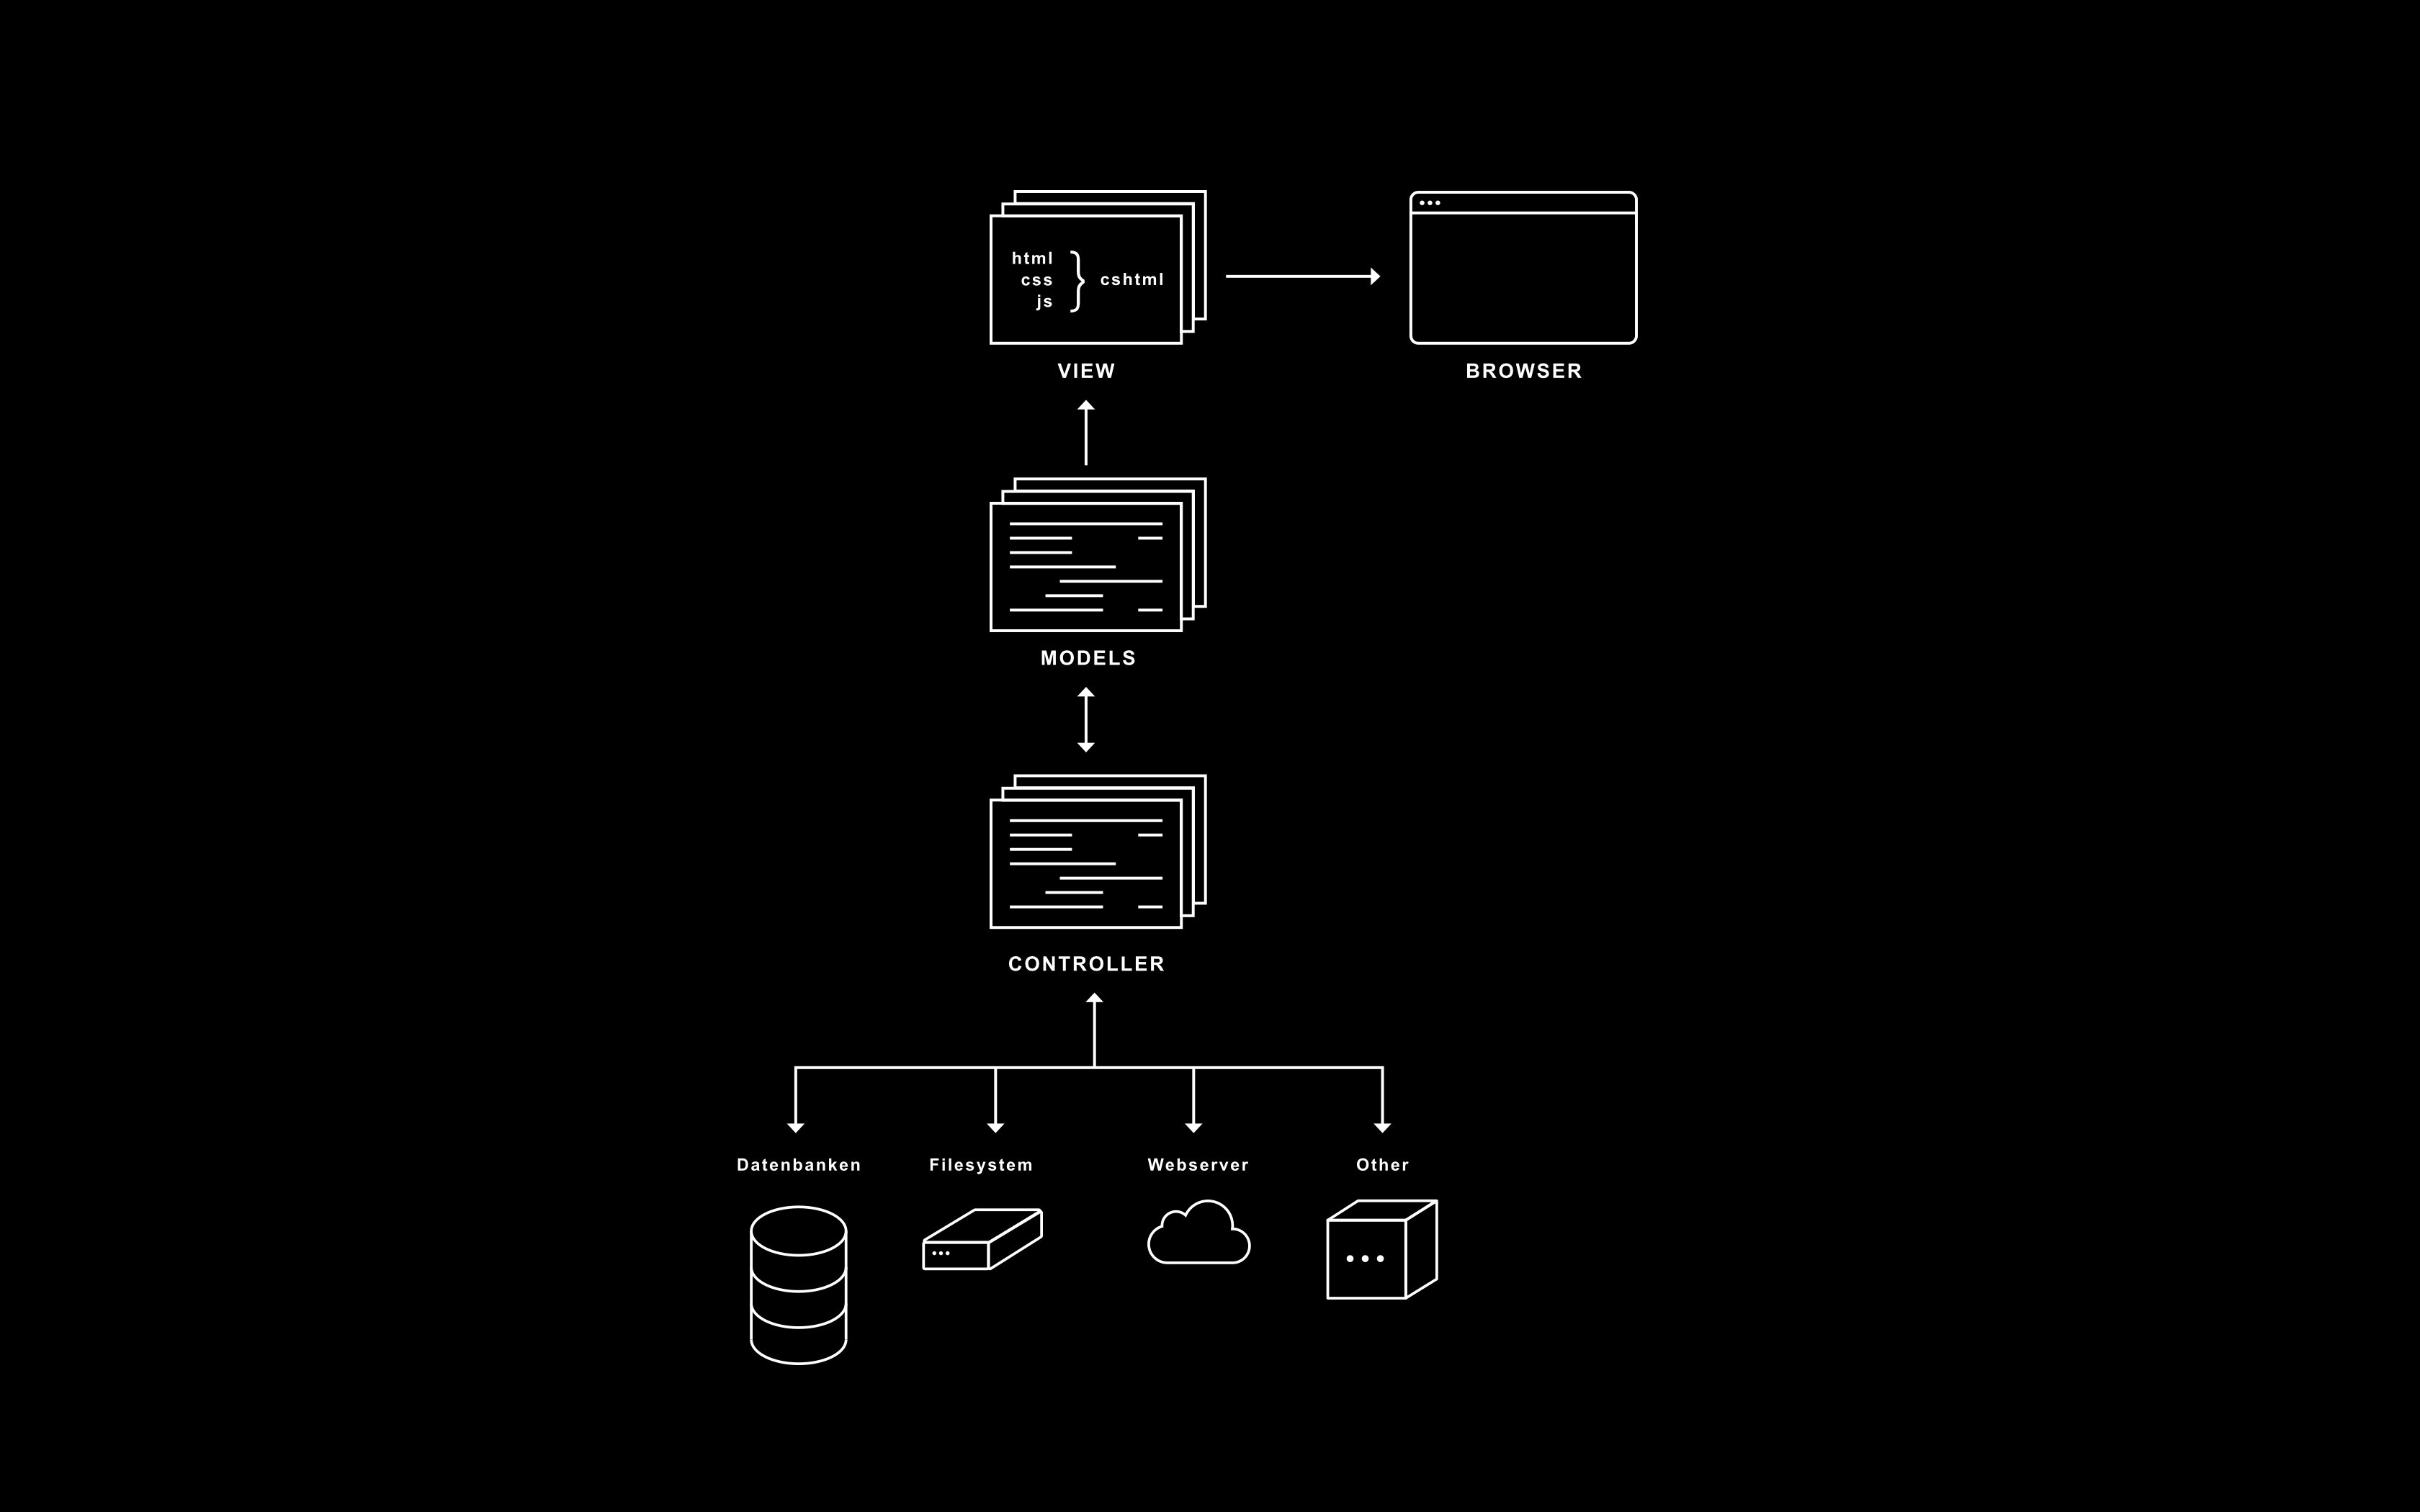
\includegraphics[width=.8\textwidth]{MVC.png}
          \caption{Model-View-Controller Pattern}
          \label{MVC}
        \end{figure}
        
        Die \textit{View}-Komponenten zur visuellen Präsentation, welche normalerweise durch HTML-Code dargestellt werden, bestehen bei ASP.Net Core aus sog. Razor-Pages.
        Das sind HTML-Dokumente, welche mittels stark typisierter Modelle eine klar definiterte Schnittstelle - die \textit{Model-Komponente} - mit dem jeweiligen Controller interagieren.

        Die \textit{Model-Komponente} sind einfache Klassen, die die grundlegende Struktur der verabeiteten Daten und der zugrundeliegenden Datenbank repräsentieren.
        Mittels Annotationen können in die Modelklasse beispielsweise Validierungen und Funktionalitäten an die Modelle angehängt werden, die vom Compiler automatisch hinzugefügt werden.
        Dadurch wird Boilerplate-Code vermieden und die Entwicklungsgeschwindigkeit erhöht.

        \textit{Controller} stellen die Businesslogik der Anwendung bereit. Das ist die Kommunikation mit dem Datenbank-Provider, Dateisystemzugriff oder die Verarbeitung von eingegeben Daten.
        Mittels Dependency-Injection können in jedem Controller zentral verwaltete Services nach Bedarf zur Verfügung gestellt werden. Das macht den Code vom Contoller leicht lesbar, selbst dokumentierend
        und reduziert ebenfalls Boilerplate-Code.

      \subsubsection{Frontend}

        Die Funktionalität unseres Frontends setzt sich aus mehreren Teilen zusammen. Die wichtigsten Elemente, welche besonderer Aufmerksamkeit bedürfen werden in diesem Absatz erläutert.

        \paragraph{Übersich der Funktionalität}

          Der übergeordnete Zweck des CMS ist die Bereitstellung und Verwaltung des Contents für die Client App. Dafür gibt es die folgenden Einzelbestandteile:

          \begin{itemize}
            \item \textit{About}-Page mit Informationen zum Projekt
            \item \textit{Upload} Bereich, wo der User sein Modell hochladen kann
            \item \textit{Showcase} Funktionalität zum Betrachten der Modelle im Browser
            \item \textit{Kurator} Bereich zur Pflege aller Metadaten
            \item \textit{Project-Pages} welche nur über einen generierten QR-Code erreichbar sind
          \end{itemize}
          
          Zur einheitlichen Einbettung dieser einzelnen Sektionen verwenden wir die Razor-Pages.

        \paragraph{Razor-Pages}

        Die zuvor erwähnte \textit{View}-Komponente wird mittels *.cshtml programiert. Das ist html-code, der durch Interoperabilität mit C\#-Modell Klassen augmentiert wurde.
        Das sieht z.B. so aus:

        \begin{lstlisting}          
          @{
            ViewData["Title"] = "Curator Area";
          }
          <h1>@ViewData["Admin"]</h1>
          <div class="text-left">
            <h1 class="display-4">Fresh Admin Panel</h1>
            <p>
                <a asp-controller="Scenes" asp-action="Create">Manage Scenes</a>
            </p>
            <p>
                <a asp-controller="StudyProgrammes" asp-action="Index">Studies Overview</a>
            </p>
            <p>
                <a asp-controller="Courses" asp-action="Index">Courses Overview</a>
            </p>
            @*<p>
                <a asp-controller="Creators" asp-action="Index">Creators Overview (Only Temporary!)</a>
            </p>*@
            <p>
                <a asp-controller="Assets" asp-action="Index">Scene Asset Table</a>
            </p>
            <p>
                <a asp-controller="Terms" asp-action="Index">Terms Overview</a>
            </p>
          </div>
        \end{lstlisting}
        
        die einzelnen Komponenten hier sind:

        \paragraph{ViewData} welche die Schnittstelle zu einem definierten \textit{ViewBag} innerhalb der C\#-Welt darstellen. Dadurch können Dropdown-Menüs o.ä. befüllt werden.
        Diese Komponenten werden durch ein vorangestelltes @-Symbol gekennzeichnet.

        \paragraph{HTML-Tags} welche wie bei gewöhnlichem HTML funktionieren. Sie reagieren auf Javascript und CSS wie bei anderen Webpages.

        \paragraph{ASP-Komponenten} werden innerhalb des *.cshtml Dokuments mit dem \textit{ASP}-Präfix gekennzeichnet. Diese elemente werden z.B. bei einem Formular in den Konstruktor
        des Datenmodells übergeben oder rufen bestimme Aktionen innerhalb des Controllers aus.
        
        \paragraph{Model Viewer}

          Eine Besonderheit innerhalb unseres Frontends stellt der Model-Viewer dar. Dieser ist ein Showcase, um die hochgeladenen Inhalte ausserhalb der Client-App bereits in der AR zu betrachten.
          Dazu verwenden wir den \textit{Google Model Viewer}\cite{ModelViewer:online}. Das ist eine kleine Javascript-Library, welches die Darstellung im Browser des Benutzers übernimmt.
          Man übergibt lediglich einen Link zum Model und je nach den Fähigkeiten des Endgeräts sind verschiedene Darstellungsarten möglich:

          \begin{figure}[H]
            \centering
            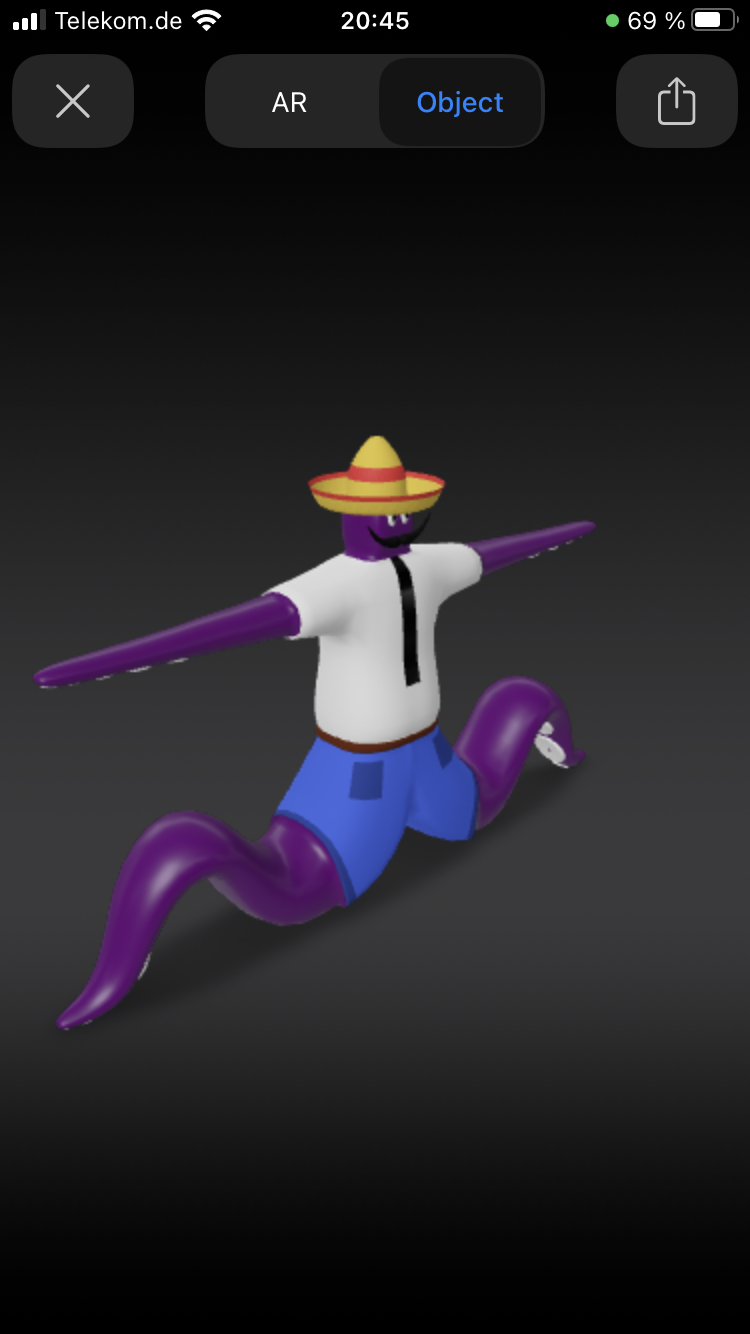
\includegraphics[width=.3\textwidth]{IMG_5810.PNG}
            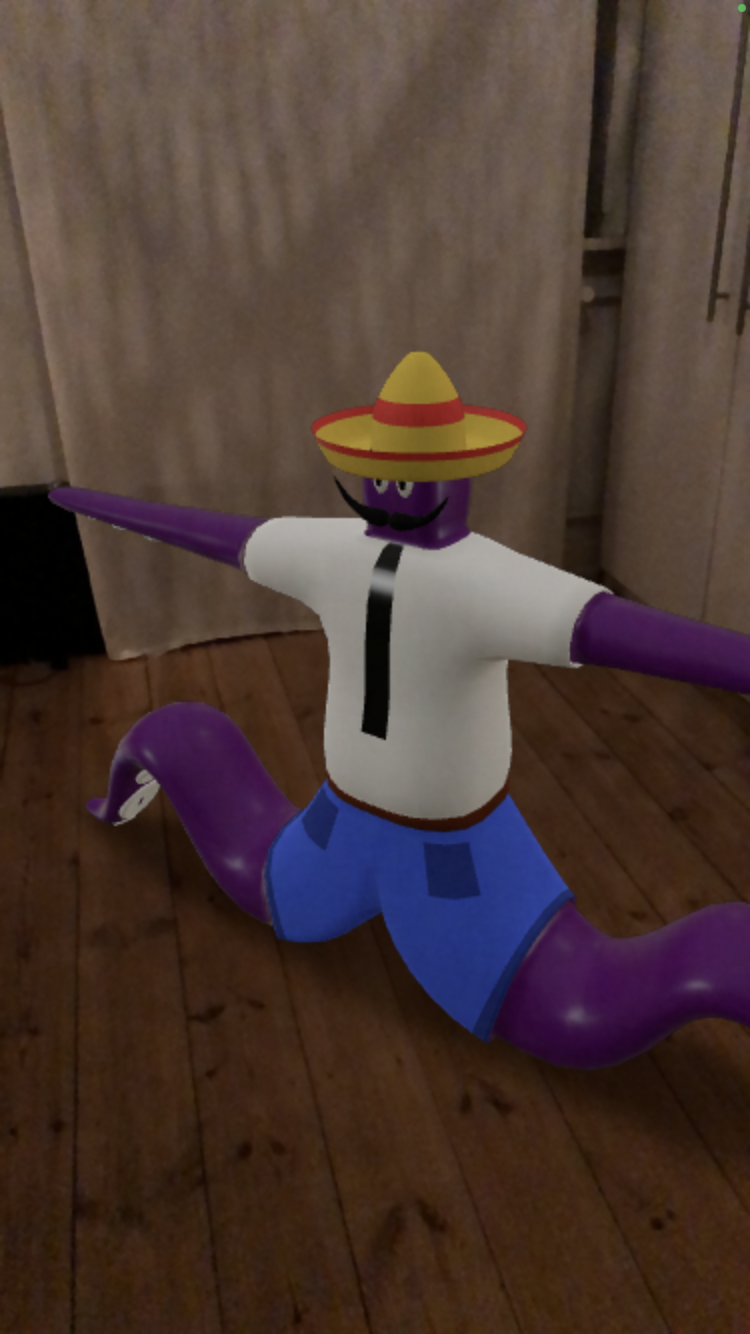
\includegraphics[width=.3\textwidth]{IMG_5811.PNG}
            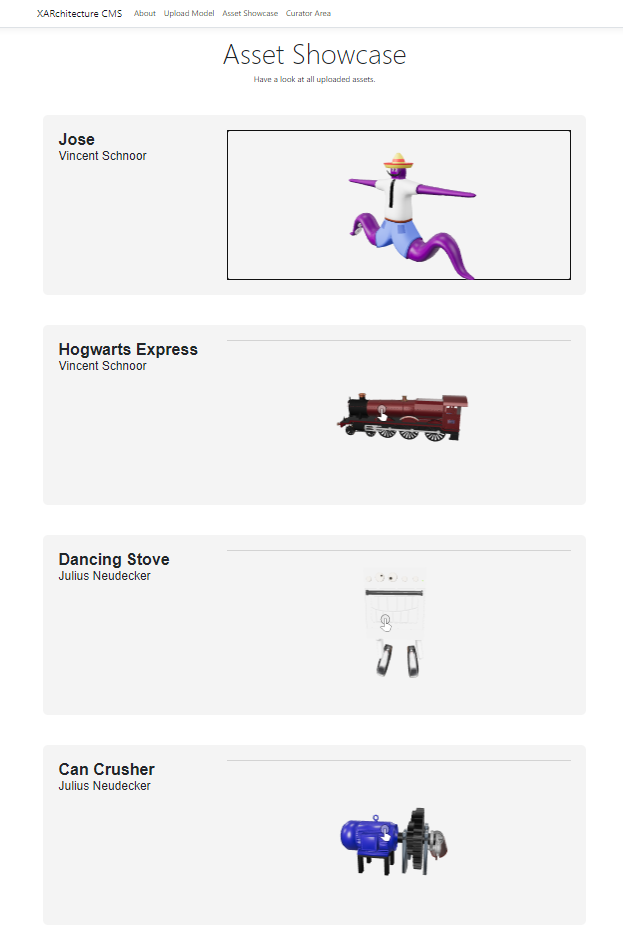
\includegraphics[width=.3\textwidth]{mv.PNG}
            \caption{Verschiedene Model-Viewer Ansichten}
            \label{ModelViewer}
          \end{figure}

          Im AR-Modus wird das Modell vom ModelViewer in der Umgebung positioniert und kann von allen Seiten betrachtet werden [1]. 
          In der Model-Only Ansicht [2] kann der Benutzer das Modell ohne die Umgebung betrachten.
          Die Desktop-Ansicht erlaubt es, mittels der Maus das Modell von allen Seiten zu betrachten.

          Ferner wird beim Upload mittels des Model-Viewers der Thumbnail\footnote{kleines Vorschaubild in Übersichten} vom User festgelegt:
          
          \begin{figure}[H]
            \centering
            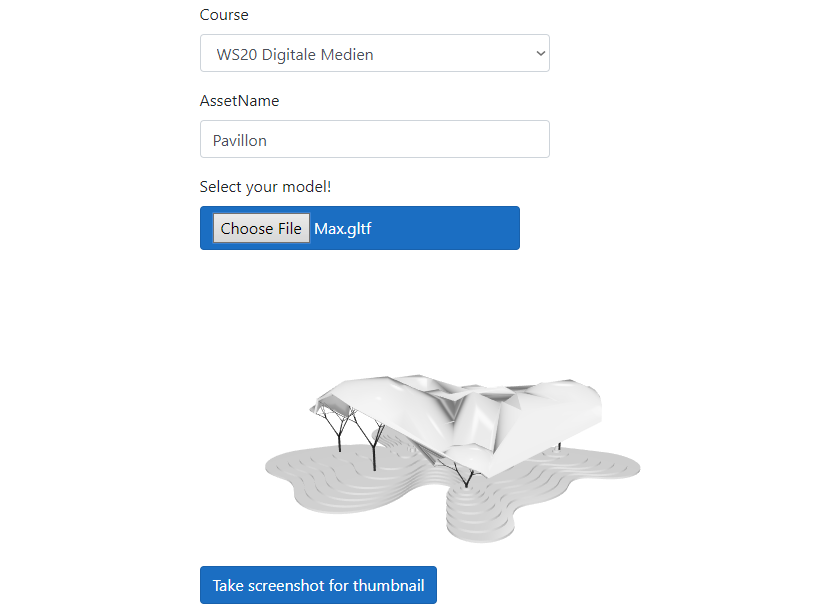
\includegraphics[width=.6\textwidth]{UploadForm.PNG}
            \caption{Upload Formular}
            \label{createThumb}
          \end{figure}

        \paragraph{Darstellung auf iOS Geräten}

          Das Dateiformat, was wir in unserer Client-App verwenden (siehe \ref{3DModel}) ist nicht kompatibel der Implementierung des ModelViewers auf iOS Geräten.
          Deswegen müssen wir für das Funktionieren dieses Features noch eine Konvertierung des 3D-Modells in das sog. \textit{USDZ}-Format\footnote{Ein proprietäres Format von Appel und Pixar} vornehmen.
          Dafür haben wir in unserer Service-Architektur einen Service im Hintergrund laufen, der sich automatisch darum kümmert.

      \subsubsection{Backend}

        Das Backend stellt alle Services bereit, die vom Frontend oder der API angefordert werden. Im Frontend selbst ist keine Logik enthalten. 
        In unserem CMS übernimmt das Backend die folgenden Aufgaben:

        \begin{itemize}
          \item Kommunikation mit der Datenbank
          \item Bereistellen der Content-API für die Client App
          \item Verwaltung des Contents auf dem Dateisystem des Hosts
          \item Erzeugen der Marker für einzelnen Szenen
          \item Darstellung der Modelle in der Showcase Sektion
          \item Hintergrundprozess zur Konvertierung in USDZ-Dateien
        \end{itemize}

        Herauszuheben sind dabei die beiden Komponenten \textit{Content API} und \textit{Dateiverwaltung}. 
        Eine ausführlichere Erläuterung der Datenbankinteraktion folgt im nächsten Kapitel.

        \paragraph{Content API} ist unsere Schnittstelle zur Client App. Dafür wird mittels eines einfachen Aufrufs über eine definierte URL\footnote{https://cms.hotpot.codes/api/content}
        im CMS ein JSON-String erzeugt, der alle notwendigen Informationen und Links zum Herunterladen der einzelnen Modelle liefert. Ein kleiner Ausschnit sähe z.B. so aus:

        \begin{lstlisting}          
          {
            "Assets": [
              {
                "Creator": {
                  "_id": "5f9a2c8f6765189948e607c2",
                  "CreatorName": "Vincent Schnoor",
                  "Assets": [
                    "5f9a2c8f6765189948e607c3",
                    "5f9a2d4a6765189948e607c4"
                  ]
                },
                "Course": {
                  "_id": "5f9a2c326765189948e607be",
                  "CourseName": "3D Modelling",
                  "StudyProgramme": "Digital Reality",
                  "Term": "SS19",
                  "University": "HAW Hamburg",
                  "Assets": [
                    "5f9a2c8f6765189948e607c3",
                    "5f9a2d7b6765189948e607c6",
                    "5f9aa9736765189948e607de"
                  ],
                  "ProgrammeNavigation": null,
                  "TermNavigation": null,
                  "UniversityNavigation": null
                },
                "AssetLinkUSDZ": "http://cms.hotpot.codes/static/content/assets/",
                "_id": "5f9a2c8f6765189948e607c3",
                "AssetName": "Jose",
                "AssetType": "3d",
                "AssetFilename": "2b9c4a6a-1e33-5bc3-aa9c-d64f5fe9d261.glb",
                "AssetLink": "http://cms.hotpot.codes/static/content/assets/",
                "ExternalLink": null,
                "ThumbnailFilename": "d994e868-3b7e-51a6-bd34-65e1d4ae917d.png",
                "ThumbnailLink": "http://cms.hotpot.codes/static/content/thumbnails/",
                "CreationDate": "2020-10-29T02:44:31.825Z",
                "Deleted": false
              },
            ...
        \end{lstlisting}    
        
        Dieser JSON-String wird auf Anfrage generiert. Die Links zum Herunterladen zeigen auf die Dateien im Dateisystem und können direkt von dort bezogen werden.

        Ferner können durch spezielle Abfragen aus der Client APP heraus bestimmte Objekte wie Szenen oder Anchors gelöscht werden. 
        Für jede Aufgabe gibt es einen definierten API-Endpoint\footnote{Der Endpoint ist eine definierte URL, über die eine gewünschte Funktionalität erreichbar ist}.

        \paragraph{Dateiverwaltung} ist wichtig für das CMS, weil dadurch die Inhalte vom Host - dem eigentlichen Stück Hardware auf dem das CMS läuft - bereitgestellt werden.
        Durch die Verwendung von Docker\footnote{Eine Virtualisierungsumgebung zur Erzeugung von leichtgewichtigen Microservices auf dem Host} sind wir Hardwareagnostisch.
        Das heisst, dass Docker hinter den Kulissen mit dem Dateisystem auf dem Host interagiert. Das von ASP.Net Core bereitgestellte Interface funktioniert unabhängig
        vom Host System immer auf die gleiche Weise. Dadurch lässt sich fehlerfreies und konsistentes Verhalten erreichen.

        Besonderes Augenmerk muss bei der Speicherung und Verwaltung der Inhalte auf Dateinamen gelegt werden. Dadurch werden Konflikte bei Dateinamen vermieden und es kann
        davon ausgegangen werden, dass jeder Dateiname einmalig ist. Das lässt sich zwar auch erreichen, indem man jeder Datei einen Zeitstempel und beliebiges Präfix zuweist.
        Effizienter und einfacher verständlich ist es aber mithilfe des Dateinamens und einem Zeitstempel einen UUID\footnote{Universally Unique Identifier} zu generieren, unter dem die Datei gespeichert wird.
        Das hat ferner den Vorteil, dass die Dateien auf dem Dateisystem anonymisiert werden. Diese UUID wird schließlich in der JSON-Api als \textit{AssetFilename} ausgegeben.       

      \subsubsection{Aufbau der Datenbank}

        Unser CMS benötigt eine Datenbank, die im Hintergrund einen persistenten Datenspeicher bereit stellt.
        Das hat gegenüber einer Speicherung in einer Textdatei oder zur Laufzeit in Datenstrukturen wie Linked Lists oder Arrays mehrere Vorteile:

        \begin{itemize}
          \item Der Datenspeicher ist eine autonome Einheit
          \item Nach Beenden des Serverprogramms bleiben die Daten erhalten
          \item Eingaben und Abfragen können einfacher abstrahiert werden
        \end{itemize}

        Wir haben uns für unser CMS für eine sog. noSQL Datenbank von MongoDB entschieden. Dabei werden Daten als \textit{Dokumente} gespeichert. 
        In MongoDB werden Datensätze als Dokumente bezeichnet. Diese kann man anschaulich mit einem JSON-String gleichsetzen, die in sog. \textit{Collections},
        also Sammlungen von Dokumenten gespeichert werden. Dabei müssen nicht alle Dokumente zwangsläufig eine identische Struktur haben.
        Der Vorteil dieser Dokumentenbasierten Speicherung ist, dass sich einzelne Dokumente durchaus unterscheiden können, sofern sie über gemeinsame Pararmeter abgefragt werden können.

        \begin{figure}[H]
          \centering
          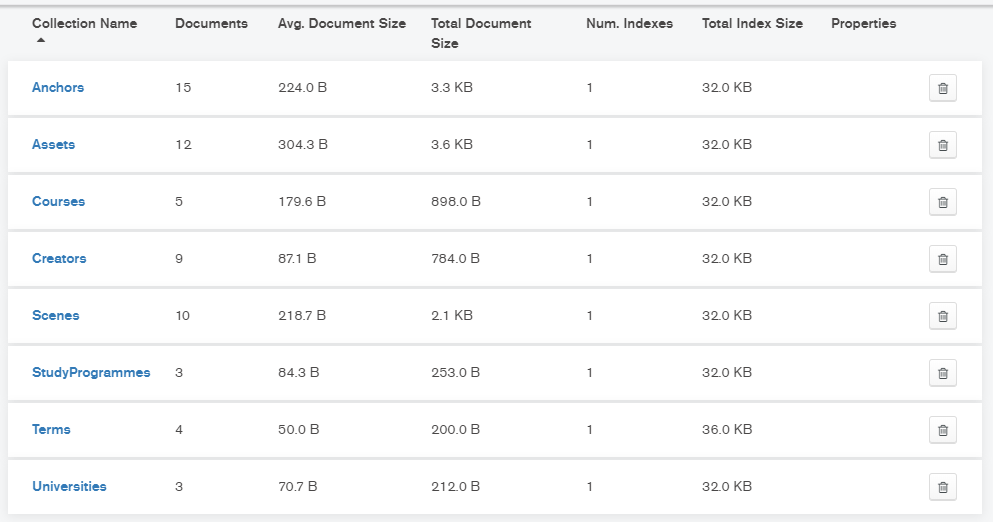
\includegraphics[width=.8\textwidth]{MongoDB.PNG}
          \caption{MongoDB Collections}
          \label{MongoCollection}
        \end{figure}

        Das hier sind alle Collections innerhalb unserer Datenbank. Jede dieser Collections speichert ein anderes Datenmodell. Im nachfolgenden Bild ist zum Beispiel die Collection für alle Assets zu sehen.
        Viele dieser Daten finden sich später im JSON-String wieder, der durch die API-Abfrage weiter oben generiert wird:

        \begin{figure}[h]
          \centering
          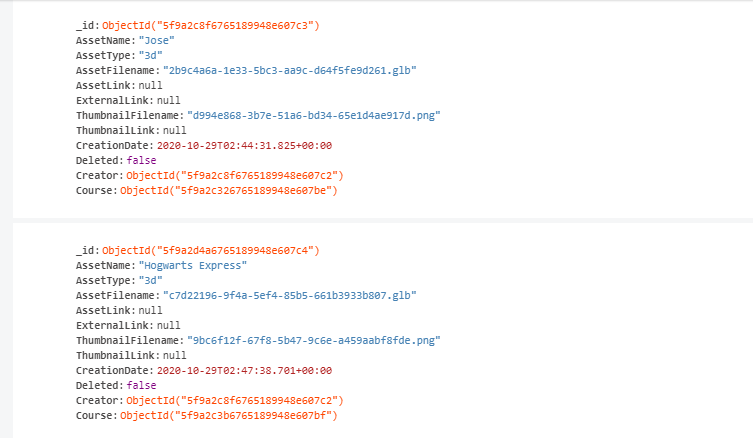
\includegraphics[width=.8\textwidth]{MongoAssets.PNG}
          \caption{MongoDB Asset Collection}
          \label{MongoAssets}
        \end{figure}

        Der große Vorteil des MVC-Patterns ist die starke Typisierung der Modelle, was eine Interaktion mit einer MongoDB stark vereinfacht.
        Die Anwendung kann bei der Verwendung eines vordefinierten Datenmodells immer darauf vertrauen, dass die Datenbank immer die geforderten Daten zurück liefert 
        und muss nichts parsen bzw. sanity checks der abgefragten Daten vornehmen.
        
        Anders als unser CMS, was wir komplett selbst programmiert haben, wird der Datenbankservice einfach mittels eines sog. \textit{Service-Providers} eingebunden
        und steht dann mittels Dependency-Injection dem entsprechenden Controller zur Verfügung. Dieser Service-Provider wird zum Start der Serveranwendung einmalig 
        konfiguriert und steht ist dann zur Laufzeit als Singleton\footnote{Einzige Instanz einer Klasse, die global erreichbar ist} erreichbar. Die Datenbank selbst ist ein Docker-Container,
        der parallel läuft und als Prozess unabhängig vom CMS ist. Der nachfolgende Code ist die Startup klasse, die alle Services definiert:

        \begin{lstlisting}          
          public void ConfigureServices(IServiceCollection services)
          {
              services.AddControllersWithViews();
              services.AddSingleton<IHttpContextAccessor, HttpContextAccessor>();
              services.AddSingleton<IFileProvider>(new PhysicalFileProvider(Directory.GetCurrentDirectory()));
  
              services.AddSingleton<IMongoClient, MongoClientBase>(s =>
              {
                  return new MongoClient(Backend.GetDatabaseConnectionString());
              });
          }
        \end{lstlisting}

        Der Singleton wird über das Interface \textit{IMongoClient} bereit gestellt bzw. bei der Instanziierung des Controllers als Dependency übergeben.
        Dadurch bleibt der Code flexibel: sollte sich die Implementierung des MongoClients verändern und das Interface gleich bleiben, müssen im Code keine Änderungen vorgenommen werden.
        Es muss lediglich die Startup-Methode angepasst werden, um bei Bedarf die Konfiguration des Singleton zu ändern.        

        \paragraph{SQL vs. noSQL}

          Ein großes Problem, was wir zu Beginn des Projektes hatten war die sich ständig verändernde Datenstruktur. Die Anforderungen und Verarbeitung der Metadaten und 
          Assets machten mehrere Revisionen der SQL-Datenbankstruktur notwendig. Das machte immer einen großen Teil des Codes obsolet, der neu geschrieben werden musste.
          SQL-Datenbanken können bei ASP.NET Core mittels des Entity Frameworks - kurz EF - als Schnittstelle verwendet werden. Dieses EF verlangte ebenfalls stark typisierte Modelle, 
          die problemlos geändert werden konnten. Ein Problem ist allerdings, dass SQL-Datenbanken genau diese Struktur auch auf Tabellenebene wiederspiegeln müssen.
          Daher muss auch jedes mal bei einer Änderung der Datenstruktur die Klasse, die mit der Datenbank interagiert - der sog. Model-Builder - neu geschrieben werden.
          
          Ein weiteres Problem ist \textit{Class-Table Inheritance}. Aus objektorientierten Programmiersprachen kennt man das Prinzip der Vererbung. 
          Hierbei können Basisklassen definiert werden, wie z.B. ein \textit{Asset}. Von dieser Basisklasse können dann wiederum weitere Klassen abgeleitet werden, 
          wie \textit{Modell} oder \textit{Video}. Diese Beziehung ist in SQL nur über Umwege über die Class-Table Inheritance möglich und stellt eher einen Workaround dar.

          noSQL-Datenbanken wie MongoDB haben dieses Problem nicht. Das stark typisierte Modell kann auch über mehrere Vererbungsstufen erstellt werden und problemlos
          mit der flexiblen Dokumentenstruktur dieses Datenbanktyps interagieren. Das hat unseren Entwicklungsprozess erheblich vereinfacht, weil es die Anpassung 
          des Datenmodells darauf reduziert hat, die Struktur im Modell und ggfs. der Businesslogik zu ändern.

      \subsubsection{Development und Integration Workflow}

        Wir haben von vornherein darauf Wert gelegt, dass wir einen Workflow implementieren, der paralleles Arbeiten an den Komponenten ermöglicht.
        Speziell im späteren Verlauf des Projektes war es wichtig, dass der App ständig eine Datenbank zur Verfügung stand, während andererseits an dieser Datenbank entwickelt wurde.
        Die Lösungen, die wir dafür in unseren Workflow implementiert haben sind State-Of-The-Art und bilden bereits im kleinen Maßstab die Arbeitsweise von großen Firmen
        ab, wo teilweise hunderte Entwickler an einer gemeinsamen Codebasis arbeiten. Das Gleiche gilt auch für das Deployment\footnote{Eine Anwendung auf einem Server starten und öffentlich erreichbar machen} 
        der Anwendung.

        Aufgrund unserer Teamgröße ist der Workflow jedoch wesentlich weniger bürokraktisch hinsichtlich Freigaben, Code Reviews und Unit Tests.

        \paragraph{Versionsverwaltung mit Git}

          Wir haben bei unserer Entwicklung stark auf Github als unser VCS\footnote{Version Control System} gesetzt. Das Vorgehen hier ist wie folgt:

          \begin{itemize}
            \item Entwickler A schreibt Code für ein neues Feature auf einem sog. Feature-Branch
            \item Entwickler A \textit{commited} diesen Code in das Repository
            \item Ist das Feature \textit{Production-Ready} wird mittels eines Pull-Requests der Code in den Master-Branch integriert
            \item Entwickler B kann sich nun den aktuellen Code aus dem Master-Branch in seinen eigenen Feature-Branch integrieren und arbeitet direkt mit dem aktuellsten Stand weiter.
          \end{itemize}

          Durch diese Arbeitsweise werden später Konflikte vermieden, wenn mehrere Entwickler parallel am gleichen Projekt arbeiten.
          Alle Entwickler arbeiten in ihrer Entwicklung in ihrem eigenen Feature-Branch, der bei Fertigstellung in den Master-Branch einfliesst.

          \begin{figure}[H]
            \centering
            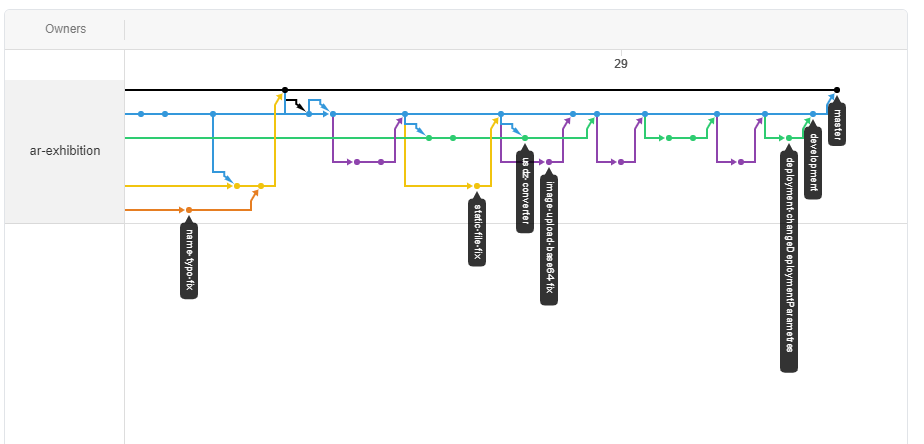
\includegraphics[width=.8\textwidth]{gitBranches.PNG}
            \caption{Netzwerk mehrerer Branches}
            \label{GitNetworks}
          \end{figure}
          
          Dabei können vor der Genehmigung von Pull-Requests auch Code-Reviews durchgeführt werden, um die Qualität des Codes zu evaluieren,
          bevor er in Produktion geht.
          
          Die Speicherung auf einem Online-Repository bietet darüber hinaus den Vorteil, dass keine Daten verloren gehen können.
          Es stellt also neben einer Versions- und Qualitätskontrolle ebenfalls ein automatisches Backup dar.

          Sollte sich also Beispielsweise ein Bug im Code einschleichen, der erst nach einiger Zeit bemerkt wird, kann die Historie
          der Commits nachverfolgt werden, um ggfs. den funktionierenden Code wiederherzustellen.

        \paragraph{Docker}

          Wie bereits erwähnt, ist Docker eine Lösung, um Anwendungen in kleine und schlanke Container zu isolieren, um sie auf einem System mit beliebigem 
          Betriebssystem auszuführen. Diese Container lassen sich mittels sog. \textit{Environment Variables} nach Bedarf schnell für eine bestimmte Umgebung konfigurieren.
          Das kann z.B. beinhalten:

          \begin{itemize}
            \item Usernamen und Passwörter für Ressourcenzugriff
            \item Netzwerkkonfiguration
            \item Development oder Production Umgebungen
            \item Datenspeicherorte auf dem Host-System
          \end{itemize}

          Dafür werden sog. \textit{Orchestration-Tools} wie Docker-Compose, Docker-Swarm oder Kubernetes verwendet. 
          Diese erlauben eine flexible Orchestrierung mehrerer voneinander abhängiger Container in einer funktionellen Einheit.
          In unserem Beispiel ist das die Backend-App, die Datenbank, der USDZ-Konverter Service und ein Service für ein automatisches Deployment.
          Das wird über ein \textit{Docker-Compose.yml} File realisiert. Diese sehen folgendermaßen aus:

          \begin{lstlisting}          
            version: '3.4'

            services:
            
              cmsProduction:
                image: ${REGISTRY_HOST}/cms:${TAG}
                container_name: cms_Frontend
                restart: always
                expose:
                  - "8080"
                environment:
                  DATABASE_HOST: ${MONGO_HOST}
                  DATABASE_REMOTE_PORT: ${MONGO_PORT}
                  DATABASE_NAME: ${MONGO_DB_NAME}
                  DATABASE_USER: ${MONGO_INIT_USERNAME}
                  DATABASE_PASSWORD: ${MONGO_INIT_PASSWORD}
                  ASPNETCORE_ENVIRONMENT: ${ASP_CONFIG}
                  USDZ_CONVERTER_HOST: ${DOCKER_HOST_USDZ}
                  USDZ_CONVERTER_PORT: ${DOCKER_PORT_USDZ}
                  VIRTUAL_HOST: ${CMS_V_HOST}
                  VIRTUAL_PORT: ${CMS_V_PORT}
                  LETSENCRYPT_HOST: ${CMS_LE_HOST}
                  LETSENCRYPT_EMAIL: ${CMS_LE_EMAIL}
                volumes:
                  - ${ASSETS}:/app/static/content/assets
                  - ${WORLDMAPS}:/app/static/content/worldmaps
                  - ${MARKER}:/app/static/content/marker
                  - ${THUMBS}:/app/static/content/thumbnails
                networks:
                  - proxy
                  - app
            
              mongo:
                image: mongo
                restart: always
                container_name: cms_Mongo
                ports:
                  - ${MONGO_PORT}:${MONGO_PORT}
                environment:
                  MONGO_INITDB_ROOT_USERNAME: ${MONGO_INIT_USERNAME}
                  MONGO_INITDB_ROOT_PASSWORD: ${MONGO_INIT_PASSWORD}
                volumes:
                  - ${MONGO_HOST_DATABASE_VOLUME}:/data/db
                networks:
                  - proxy
                  - app
                  
              watchtower:
                image: containrrr/watchtower
                container_name: cms_Watchtower
                volumes:
                  - /var/run/docker.sock:/var/run/docker.sock
                  - /root/.docker/config.json:/config.json
                command: --interval 30
                
              usdz:
                image: marlon360/gltf-to-usdz-service:latest
                container_name: cms_USDZ
                labels:
                  com.centurylinklabs.watchtower.enable: "false"
                volumes:
                  - ${ASSETS}:/usr/app
                networks:
                  - app
            
            networks:
              proxy:
                external:
                  name: nginx-proxy
              app:
            
          \end{lstlisting}

          Ohne auf jedes Detail einzugehen, sind einige wichtige Komponenten nennenswert: Die jeweiligen Container werden unter \textit{services} mit ihrer jeweiligen Konfiguration aufgelistet.
          Unter \textit{environment} werden die bereits erwähnten Environment Variables definiert. Diese liegen zur einfachereren Verwaltung und aus Sicherheitsgründen in einer \textit{.env}-Datei
          im gleichen Verzeichnis und werden von Docker beim Start ausgelesen. Ferner werden für jeden Container definierte Namen zugewiesen. Weil solch ein Compose-File immer alle Services startet,
          können funktional zusammenhängende Services in diesen Dateien gemeinsam konfiguriert werden.

          \begin{figure}[H]
            \centering
            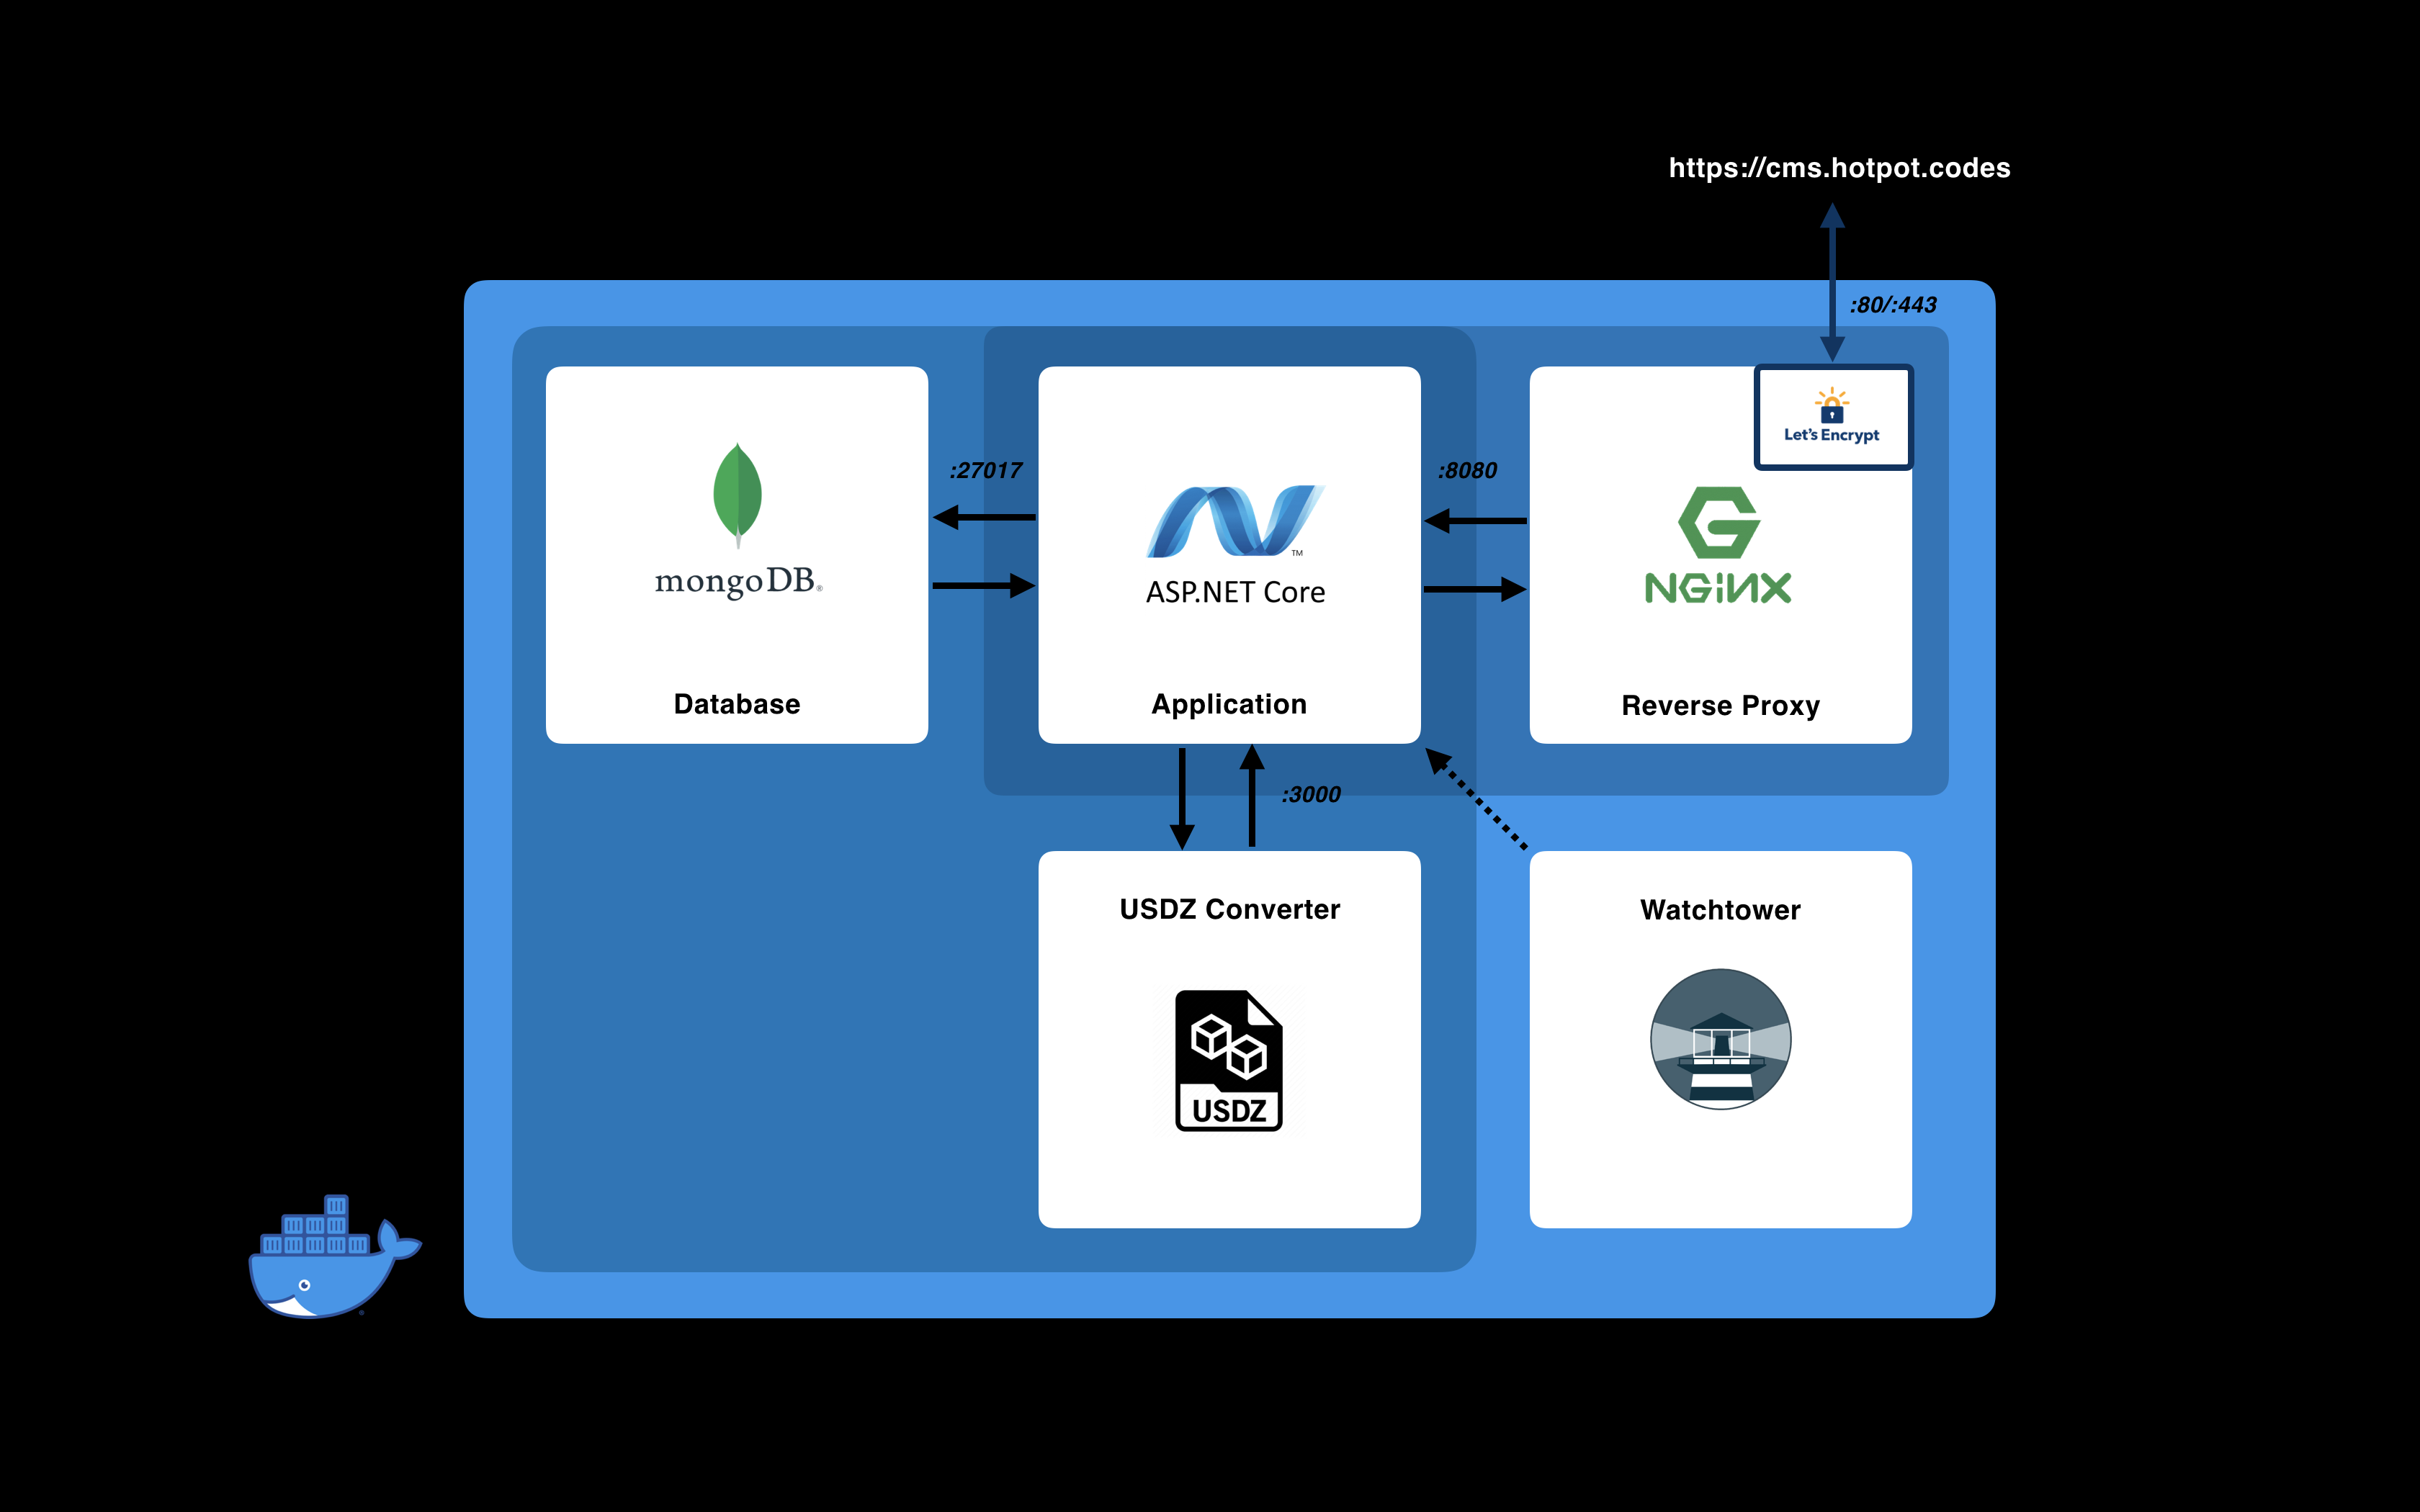
\includegraphics[width=.8\textwidth]{DCompose.png}
            \caption{Docker Container Orchestrierung}
            \label{pipeline}
          \end{figure}

        \paragraph{Deployment}        

          Die Fäden laufen zusammen bei sog. \textit{Github Actions}. Das sind Programme, die auf dem Repository ausgeführt werden, wenn bestimmte Bedingungen erfüllt sind.
          In unserem konkreten Fall werden diese getriggert, wenn Code in den Master-Branch eingefügt wird. Diese Actions bauen dann das Docker-Image und laden es auf unsere interne
          Docker-Registry hoch. Der in der Docker-Compose ausgeführte \textit{Watchtower} prüft in regelmäßigen Abständen, ob sich das Docker-Image geändert hat und triggert in diesem Fall
          den Deployment-Prozess. Dazu wird das neue Image heruntergeladen, der jeweilige Container \textit{gracefully}\footnote{Eingehende Client-Verbindungen und Schreibprozesse werden kontrolliert beendet.} 
          beendet und anschließend mit dem neuen Image wieder gestartet. Da im Idealfall keine Anpassung der Konfiguration notwendig ist, kann dieser Prozess komplett automatisiert erfolgen.
          Der jeweilige Verantwortliche macht nur den Pull-Request auf den Master Branch und alle weiteren Schritte erfolgen dann automatisch und nach wenigen Minuten ist das neue Release veröffentlicht.

          Das bietet einen standardisierten Workflow, der effizient und weniger fehleranfällig ist als die klassische Methode, wo ein Administrator eine neue Version in den Systemkontext einbetten und
          dann starten musste. Moderne Tools wie \textit{Puppet} oder \textit{Chef} machen das zwar ebenfalls einfacher aber eine Container-Lösung ist diesem Vorgehen in vielerlei Hinsicht überlegen.

          \begin{figure}[H]
            \centering
            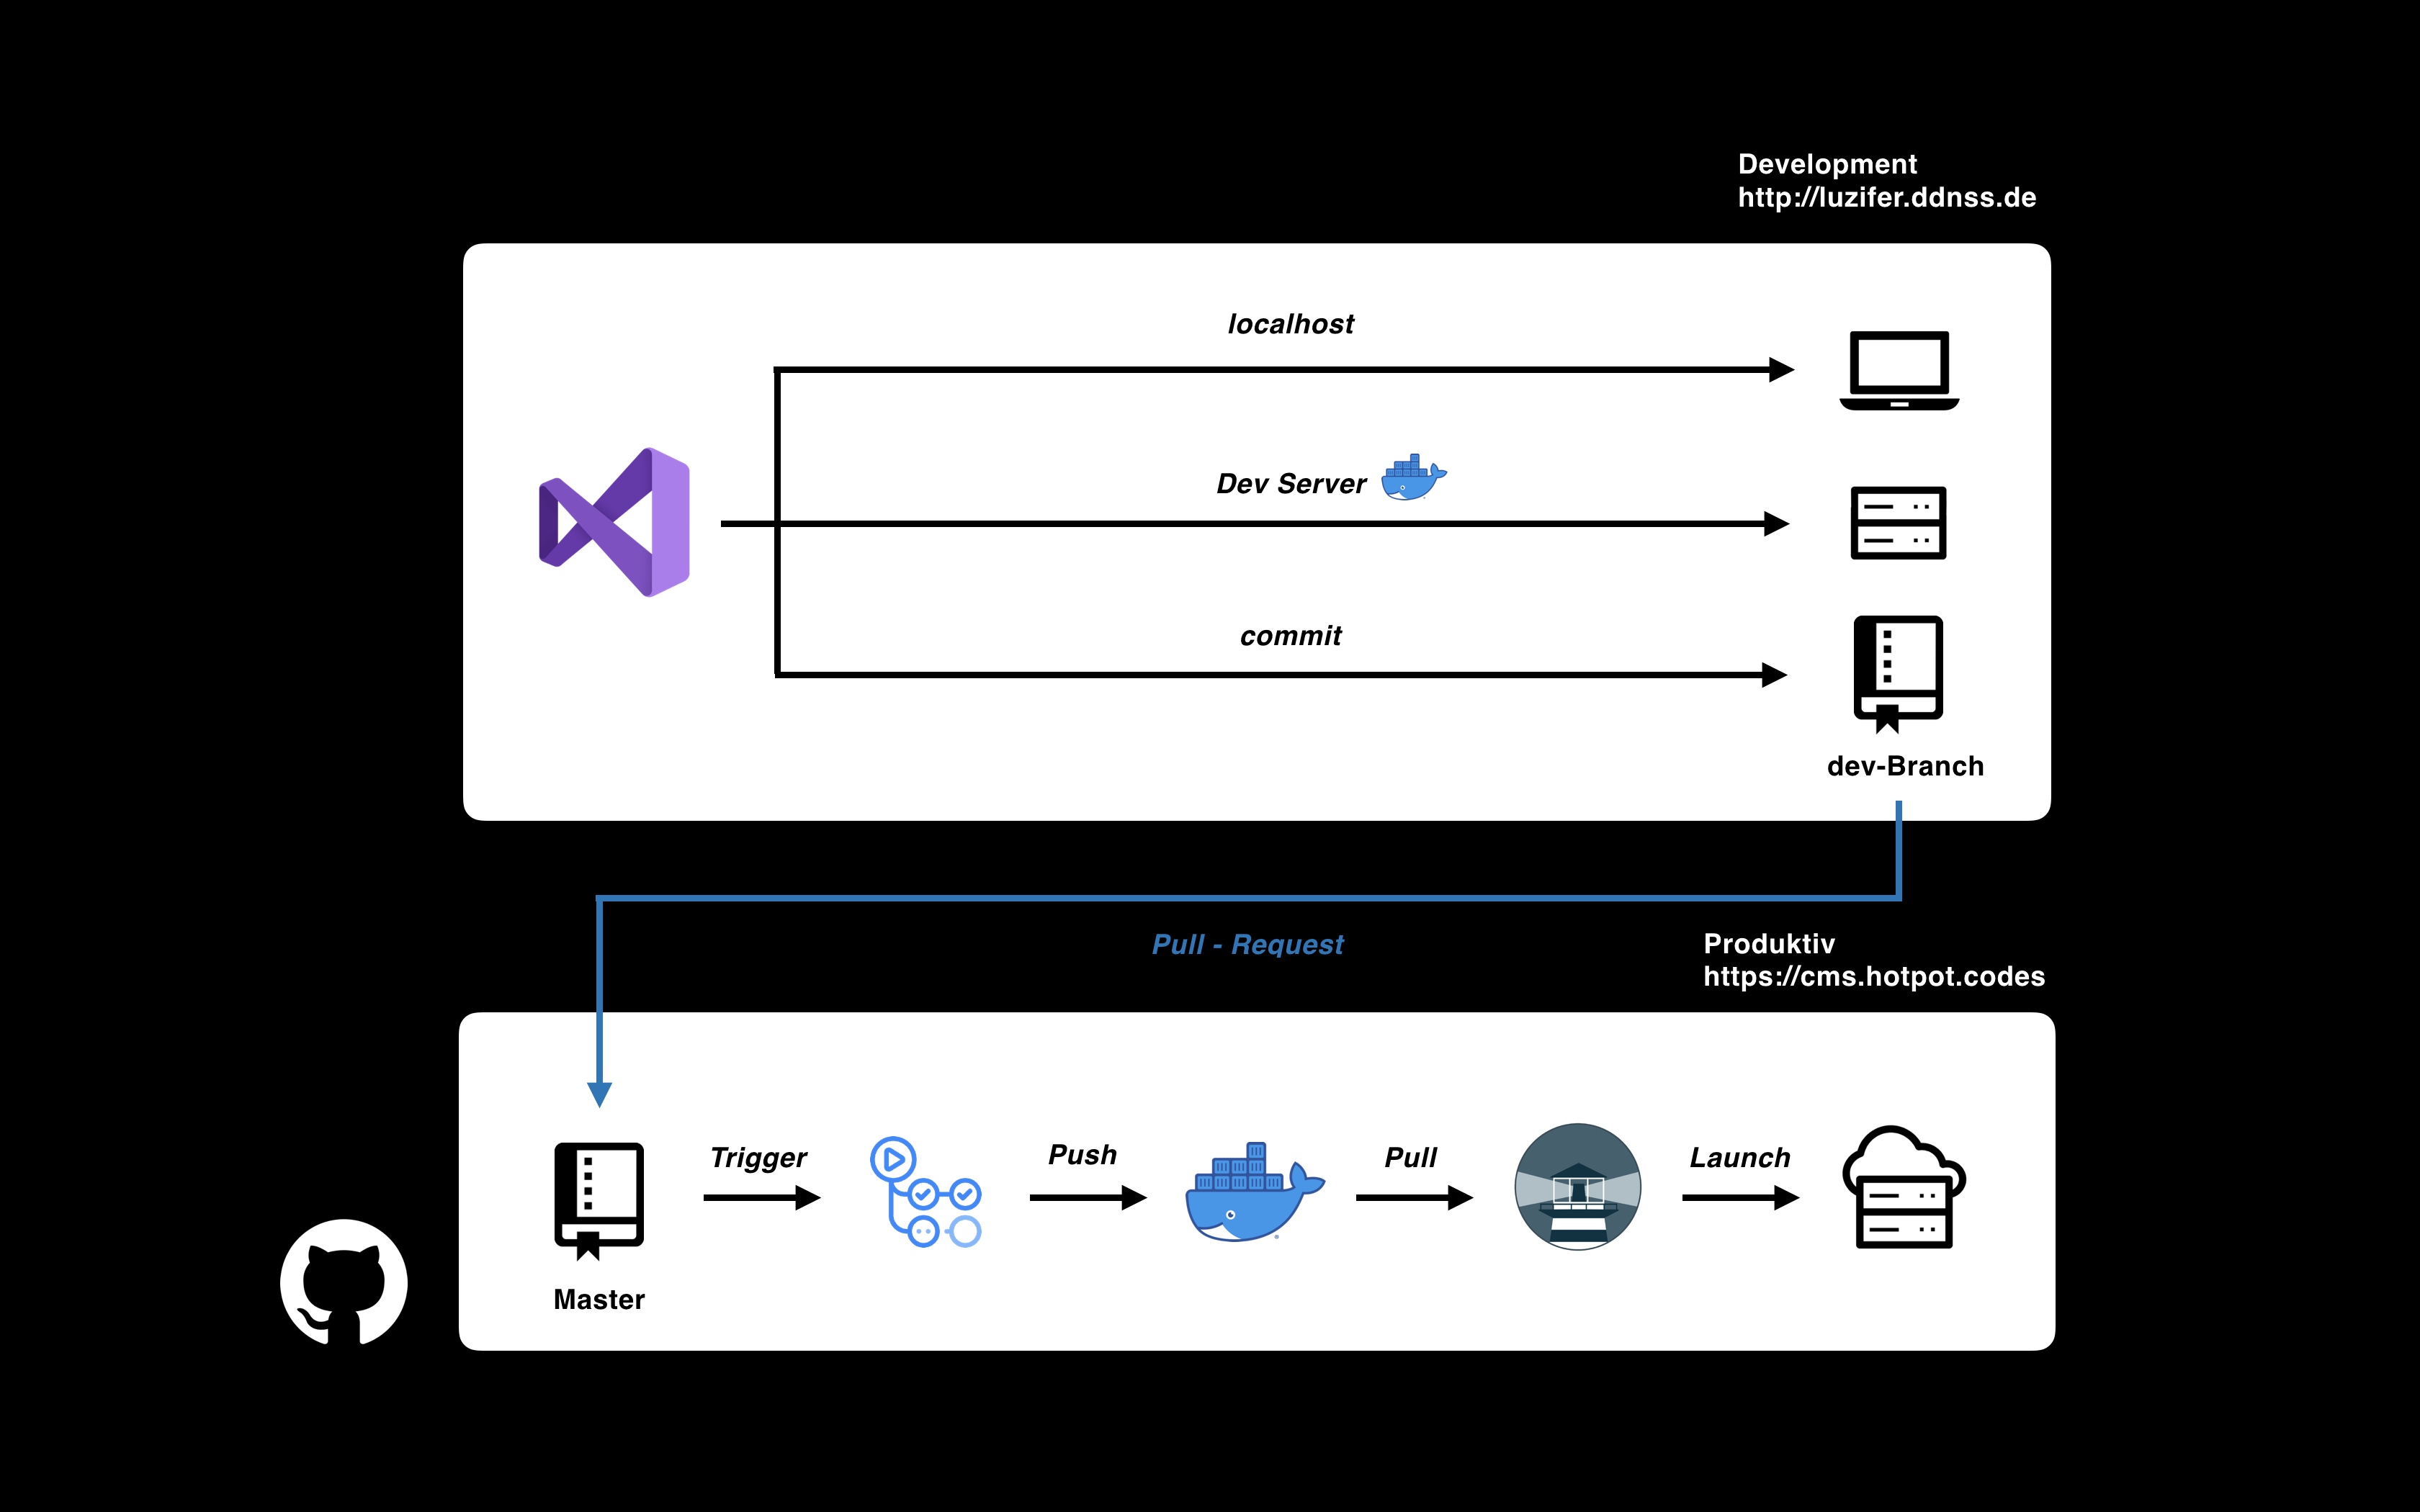
\includegraphics[width=.8\textwidth]{pipeline.png}
            \caption{Development Workflow}
            \label{pipeline}
          \end{figure}

        \paragraph{Test vs. Production}

          In der Entwicklung hatten wir etwa ab der Mitte des Projekts das Problem, dass für die Entwicklung der App das Backend ständig verfügbar sein musste.
          Wird parallel an dem Backend gearbeitet, ist das allerdings nicht immer möglich, weil Bugs oder neue Features häufig zu einer nicht-Verfügbarkeit führen.
          Daher sind wir relativ frühzeitig auf ein zweigleisiges Modell umgestiegen, wo es einen Development- und einen Production-Server gibt. 
          Ersterer konnte vom Entwickler bei Bedarf das neue Image starten und ermöglichte Debugging und Testen ohne die Entwicklung der App zu beeinträchtigen.
          War die implementierung des neuen Features \textit{Production Ready}, konnte der Deployment-Prozess gestartet werden und der neue Code wurde dann auf dem Production
          Server deployed. Außerdem werden an einen Produktionserver ganz andere Anforderungen hinsichtlich Netzwerkbandbreite, Verfügbarkeit und Performance gelegt.
          Dieser muss im Zweifelsfall eine große Menge User bedienen können. Der Development Server hat nur schlimmstenfalls nur einige wenige User und wird nur von den Entwicklern verwendet.
          Das ist neben der bereits erwähnten Verfügbarkeit für die App Entwicklung auch kosteneffizienter, weil spezialisierte Maschinen verwendet werden können.

    \subsection{AR App}

    \subsubsection{Verwendung von 3D-Modellen}\label{3DModels}
    
    Da die Platzierung von 3D-Modellen ein Hauptbestandteil der App ist, wurde ein großer Fokus auf das Dateiformat der 3D-Modelle gelegt. Die dynamische Verwendung der Modelle in der App sollte möglichst einfach und problemlos sein.\\ 
    Aus diesem Grund wurden die verschiedenen von Unity unterstützten Dateiformate miteinander verglichen, um die im Dateiformat unterstützten Funktionalitäten und die Qualität der Darstellung in der App zu vergleichen.\\
    Unity unterstützt nativ die folgenden Dateiformate:
    \begin{itemize}
    \item FBX
    \item DAE (Collada)
    \item DXF
    \item OBJ
    \end{itemize}
    Da die meisten Studenten Blender als 3D-Modelling Tool ihrer Wahl nutzen wurde ein Vergleich der in Blender möglichen Export-Dateiformate und der in Unity unterstützten Formate gemacht. Blender exportiert 3D-Modelle unter anderem als FBX und OBJ, welche ohne großen Aufwand in Unity importiert werden können.\\
    Der Nachteil dieser Formate ist, dass die Materialien und Texturen als externe Dateien in einem getrennten Ordner exportiert werden. Für die direkte Verwendung in Unity kein Problem erschwert dies jedoch das Zwischenspeichern in unserem Content-Management-System. Weiterhin werden \glqq Faces\grqq, Flächen eines 3D-Modells, mit mehr als 5 \glqq Vertices\grqq, Eckpunkten, nicht unterstützt und somit in Unity nicht dargestellt. Bei nicht komplett sauber erstellten 3D-Modellen können so unschöne Lücken im Modell entstehen die unerwünscht sind.\\
    Aus diesem Grund wurde das von der Khronos Group entwickelte und in Blender integrierte GLTF 2.0 Format auf seine Verwendbarkeit in Unity untersucht. GLTF speichert sämtliche Daten eines 3D-Modells, darunter auch Materialien und Animationen, in einer einzigen, auf dem JSON-Dateiformat basierenden Datei ab. Das Dateiformat ist extrem robust und speichert jegliche Geometrie eines 3D-Modells ab. Der Nachteil des GLTF-Formates ist allerdings, dass dieses erst ab der Blender Version 2.81 unterstützt und erst ab 2.83 richtig implementiert ist. Alte Blender Modelle müssen demnach auf eine höhere Blender-Version gebracht und dort exportiert werden. Weiterhin unterstützt Unity, wie in der Auflistung oben zu sehen, das Dateiformat GLTF 2.0 nicht nativ, weshalb zusätzliche Bibliotheken benötigt werden um die Dateien nutzen zu können.\\
    Eine dieser und die in unserem Projekt verwendete Bibliothek ist die \textit{GLTFUtility} Bibliothek des GitHub-Nutzers \textit{Siccity}. \textit{GLTFUtility} unterstützt den Import und Export von GLTF Dateien in Unity während der Laufzeit, was für unser Projekt von elementarer Bedeutung ist, da die 3D-Modelle beim Starten der App nicht bereits vorliegen, sondern während der Laufzeit der App dynamisch geladen und verwendet werden.\\

    Der Vergleich der drei untersuchten Dateiformate hinsichtlich Qualität zeigte, dass die Darstellung von GLTF-Modellen gegenüber FBX- und OBJ-Modellen besser ist (siehe Abbildungen x, y und z). Die von Blender exportierten Materialien werden im GLTF-Format, durch die bessere Unterstützung diverser Material-Eigenschaften, besser dargestellt.\\

    Aus diesen Gründen, der besseren Darstellung der 3D-Modelle in Unity, die robustere Geometrie-Darstellung und der Export in einer einzigen Datei, entschieden wir uns dazu GLTF als einziges Dateiformat für die Verwendung innerhalb der App zu verwenden.
    \subsubsection{Export-Anforderungen an 3D-Modelle}
    Die im Laufe des Projektes erstellten Anforderungen an den Export der 3D-Modelle hinsichtlich ihrer Material-Eigenschaften und Animationen beziehen sich ausschließlich auf den Export in der 3D-Modelling-Software Blender.\\

    Die in Blender erstellten Materialien weisen mit zunehmender realitätsnähe eine steigende Komplexität auf. Aus diesem Grund mussten bestimmte Anforderungen an den Export von 3D-Modellen aus Blender gestellt werden, um die korrekte Darstellung in der von uns entwickelten App zu gewährleisten. Die folgenden Anforderungen gelten für den Export von 3D-Modellen aus Blender um die Darstellung in unserer App zu gewährleisten.\\

    \textbf{Meshes:}\\
    GLTF unterstützt den Export von jeglicher Geometrie des Meshes. Dabei ist die Anzahl der Vertices eines Faces irrelevant, da Quads und N-Gons beim Export automatisch in Triangles umgewandelt werden.\\
    Kurven und andere \glqq Nicht-Mesh\grqq Daten werden nicht übernommen uns müssen vor dem Export in Meshes umgewandelt werden.\\

    \textbf{Materialien:}\\
    GLTF unterstützt die folgenden Material-Eigenschaften beim Export:
    \begin{itemize}
    \item Base Color
    \item Metallic
    \item Roughness
    \item Baked Ambient Occlusion
    \item Normal Map
    \item Emissive
    \end{itemize}
    Texturen werden als Base Color problemlos unterstützt. Bei Roughness und Metallic Texture-Maps müssen einige Einstellungen vor dem Export getroffen werden. Bei einer Textur erwartet GLTF die Metallic-Werte kodiert im B-Farbchannel, während die Roughness-Werte im G-Farbchannel kodiert sind. Das Node-Setup in Blender sollte demnach folgendermaßen aussehen:\\
    %Bild einfügen
    Wurde das Node-Setup nicht angepasst wird versucht beim Export die relevanten Daten auszulesen, was mitunter zu längeren Exportzeiten führen kann.\\
    Baked Ambient Occluion, Normal Maps und Emissive Materials werden problemlos unterstützt und müssen nicht weiter angepasst werden.\\

    \textbf{Animationen:}\\
    Animationen im GLTF-Format zu exportieren ist nicht kompliziert. Folgende Animationstypen werden nativ beim Export unterstützt:
    \begin{itemize}
    \item Keyframes (Translation, Rotation, Scale)
    \item Shape Keys
    \item Armatures/Skinning
    \end{itemize}
    Animationen anderer Eigenschaften wie Licht oder Materialien werden ignoriert.\\
    Wenn das 3D-Modell nur eine Animation hat gibt es bei der Verwendung in Unity keine Probleme. Probleme entstehen wenn das 3D-Modell aus mehreren Einzelteilen besteht die jeweils eigene Animationen haben, da die Animationen in Unity im Legacy Animation-System abgespielt werden müssen, welches nur eine Animation zur Zeit unterstützt. Aus diesem Grund müssen mehrere Animationen einem NLA Track hinzugefügt werden. Dieser dient quasi als Animations-Controller, welcher die einzelnen Animationen zu einer einzigen Animation zusammenfasst und die verschiedenen Objektteile bewegt.\\
    Objekt-Constraints, wie \glqq Copy Location\grqq können ebenfalls exportiert werden, wenn diese vorher in Keyframes umgewandelt wurden.\\
    Die letzte Anforderung beim Export von 3D-Modellen mit mehreren Einzelteilen und Animationen ist, dass es nur \textbf{ein} Parent-Objekt geben darf. Dies kann ein leeres Objekt sein, da dies für die Hierarchy in Unity und die Verwendung der Animationen relevant ist.\\

    Wenn diese Anforderungen eingehalten werden können Blender-Modelle exportiert und in unserer App verwendet werden.

    \subsubsection{Speichern und Wiederherstellen der Einrichtung eines Raumes}

    Eine wichtige Funktion der App ist es, dass man in einem beliebigen Raum Assets platzieren kann und die Position, Rotation und Skalierung der einzelnen Assets speichern kann.
    Weitere User der App können dann die Assets exakt so wiederherstellen, wie sie vorab gespeichert wurden.

    Das zu lösende Problem besteht darin, dass beim Starten einer Augmented Reality Session immer ein neues Koordinatensystem angelegt wird.
    Der Ursprung dieses Koordinatensystems liegt immer bei der Position des AR Gerätes beim Start der App.
    Wenn nun also verschiedene Nutzer in unterschiedlichen Positionen im Raum starten, führt es dazu, dass die Assets nicht an der selben Position sind wie zuvor beim Speichern.
    
    Auf dieses Problem stößt man vor allem, wenn man sich mit dem Thema \textit{Indoor Navigation} beschäftigt. Hier muss die Navigation perfekt auf den realen Raum angepasst werden, damit die Navigation überhaupt funktionieren kann.
    Unsere App bewegt sich in der gleichen Problemdomäne, da die Assets für jeden Nutzer an der selben Position im realen Raum verankert sein müssen.

    Für dieses Problem gibt es unterschiedliche Lösungsansätze:

    \paragraph{GPS}
    GPS ist eine häufig eingesetzte Technologie für die Positionserkennung. Da es eine globale Standortermittlung ist, sind die Position für alle Nutzer ähnlich.
    Diese Technologie ist aber zu ungenau, vor allem beim Tracking innerhalb von Gebäuden. Auch ist es schwierig Stockwerke zu unterscheiden.

    \paragraph{Beacons}
    In der Indoor Navigation sind Beacons ein gute Möglichkeit einen Standort zu ermitteln. Beacons sind Geräte, die über Bluetooth eine Verbindung zu dem AR Geräte herstellen und so ermitteln können, wo sich ein Gerät befindet.

    \begin{figure}[h]
      \centering
      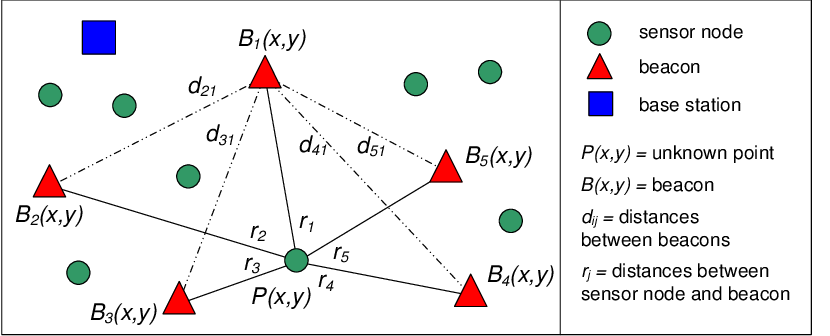
\includegraphics[width=.6\textwidth]{beacons}
      \caption{Positionsermittlung mit Beacons \cite{beaconNetwork}}
      \label{Beacons}
    \end{figure}

    In Abbildung \ref{Beacons} ist zu sehen, dass sich die Beacons (rot) an einer bekannten Position befinden. Die unbekannte Position (grün) wird durch die Abstände zu den einzelnen Beacons errechnet.

    Ein berühmtes Beispiel für den Einsatz von Beacons ist der Flughafen Gatwick in London. Hier wurden 2000 Beacons installiert, um die Indoor Navigation zu ermöglichen. \cite{GatwickA64:online} 
    Dieses System bietet eine Genauigkeit von +/- 3 Metern.
    
    Dies ist zu unganau für unsere Einsatzzwecke, da wir Assets mit der höchsten Genauigkeit platzieren und wiederherstellen möchten. Die Assets müssen sich genau in die Umgebung einbinden lassen.
    Ein Beispiel wäre die Platzierung eines 3D Objekts auf einem realem Sockel. Wenn die Ungenauigkeit bei mehreren Metern liegt, kann nicht gesichert sein, dass das 3D Objekt immer sich genau auf dem Sockel befindet.

    Des Weiteren müssen diese Beacons gekauft werden für etwas 5 - 20 Euro pro Stück und in jedem Raum installiert werden, der unsere App nutzen möchte.
    Es darf auch nicht vergessen werden, dass diese Geräte batteriebetrieben sind und somit nach 1-2 Jahren ein Wechsel der Batterien durchgeführt werden muss. 

    \paragraph{Image Markers}

    Eine weitere Möglichkeit um die Positionen der echten Welt mit der AR Welt zu synchronisieren sind \textit{Image Marker}. Meist werden Image Marker dazu genutzt 3D Objekte direkt mit einem Bild zu verankern, wie zum Beispiel bei AR Visitenkarten.
    Es ist aber auch möglich Objekte relativ zu einem Bild mit einem größerem Abstand zu platzieren. Denn wenn ein Bild mit einem AR SDK wie ARKit oder ARCore erkannt wird, wird die Position und Rotation des Bildes in der AR Session bestimmt.
    Wenn die Asset Positionen gespeichert werden, muss dies also relativ zu dem Image Marker passieren. Dazu muss immer ein Bild in einem Raum platziert werden und die Position des Bildes darf sich nicht mehr ändern, da sich sonst alle platzierten Assets ändern würden.
    Die Genauigkeit ist auf Millimeter genau. \cite{HowAugme98:online}
    
    Dennoch sinkt die Genauigkeit je weiter man sich von dem Marker entfernt.

    \begin{figure}[h]
      \centering
      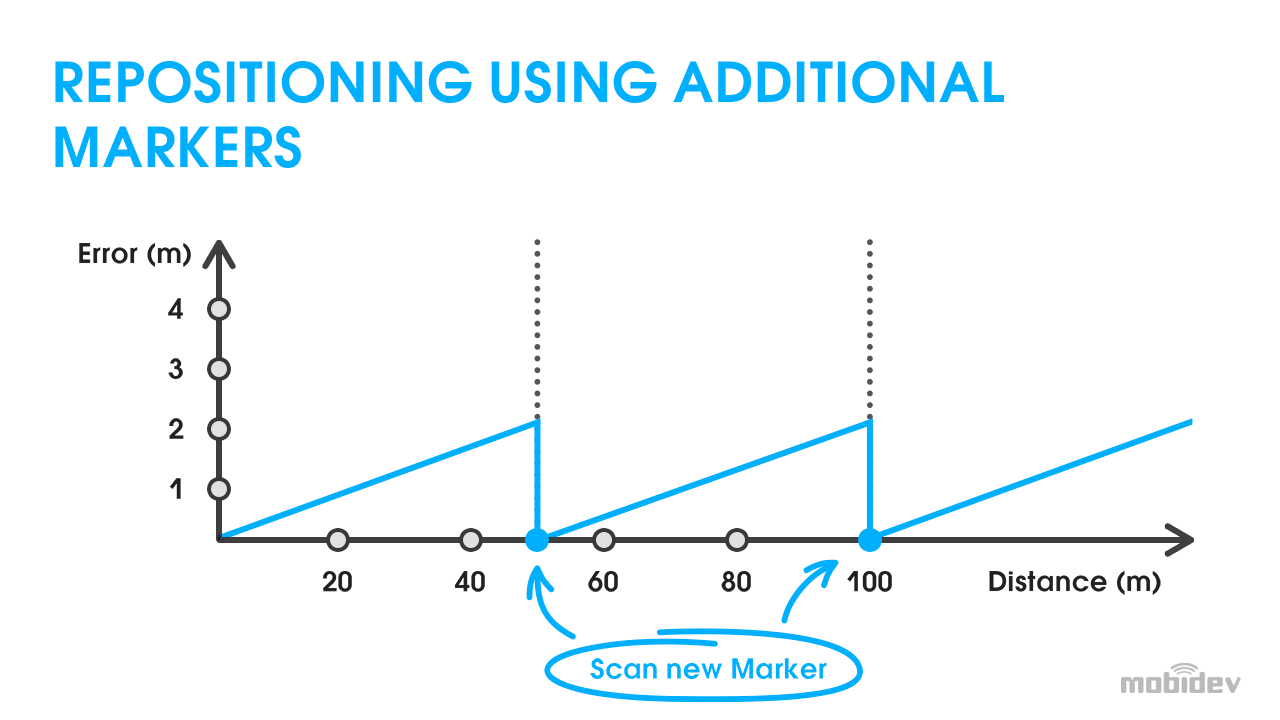
\includegraphics[width=.6\textwidth]{multi-marker}
      \caption{Repositionierung mit mehreren Image Markern \cite{HowAugme98:online}}
      \label{MultiMarker}
    \end{figure}

    In Abbildung \ref{MultiMarker} ist ein Beispiel einer Indoor Navigation zu sehen, die den Fehlerwert in Meter abhängig von der Distanz zu dem Image Marker zeigt.
    Hier wird mit mehreren Markern gearbeitet, um die Genauigkeit zu erhöhen.

    Der Vorteil dieses Ansatzes ist, dass die Genauigkeit im Bereich der Image Marker sehr hoch ist und die Marker günstig und einfach produziert werden können und ohne Strom betrieben werden.

    Der Nachteil ist, dass mit mehreren Markern gearbeitet werden muss, damit die Qualität dauerhaft gesichert werden kann. Auch muss bei der Positionierung des Markers darauf geachtet werden, dass sich die Position nicht mehr ändert.

    \paragraph{Visual Positioning System}

    Eine weitere Möglichkeit ist es eine Umgebung anhand von Referenzpunkten zu synchronisieren.
    Ein bekanntes Beispiel dieses \textit{Visual Positioning Systems} ist die AR Funktionalität von Google Maps.
    
    \begin{figure}[h]
      \centering
      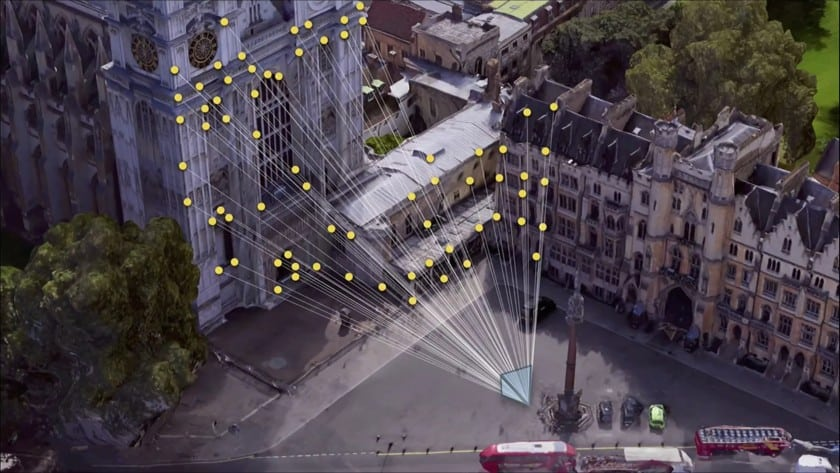
\includegraphics[width=.5\textwidth]{vps-google}
      \caption{VPS in Google Maps \cite{GoogleMa12:online}}
      \label{VPSGoogle}
    \end{figure}

    Bei Google Maps werden die Bilddaten der AR Kamera mit den Daten der Google Streetview Aufnahmen verglichen.
    Durch die Synchronisierung besonders markanter Stellen in der Umgebung (\textit{Feature Points}) kann die Position und Rotation in der realen Welt sehr genau wiederhergestellt werden.

    In Abbildung \ref{VPSGoogle} ist zu sehen wie anhand von Feature Points die Position der Kamera bestimmt wird.

    Das gleiche Prinzip kann auch auf Räume angewandt werden. Dazu werden zunächst die Feature Points aus einem Raum extrahiert und bei der Wiederherstllung wieder abgeglichen.

    \begin{figure}[h]
      \centering
      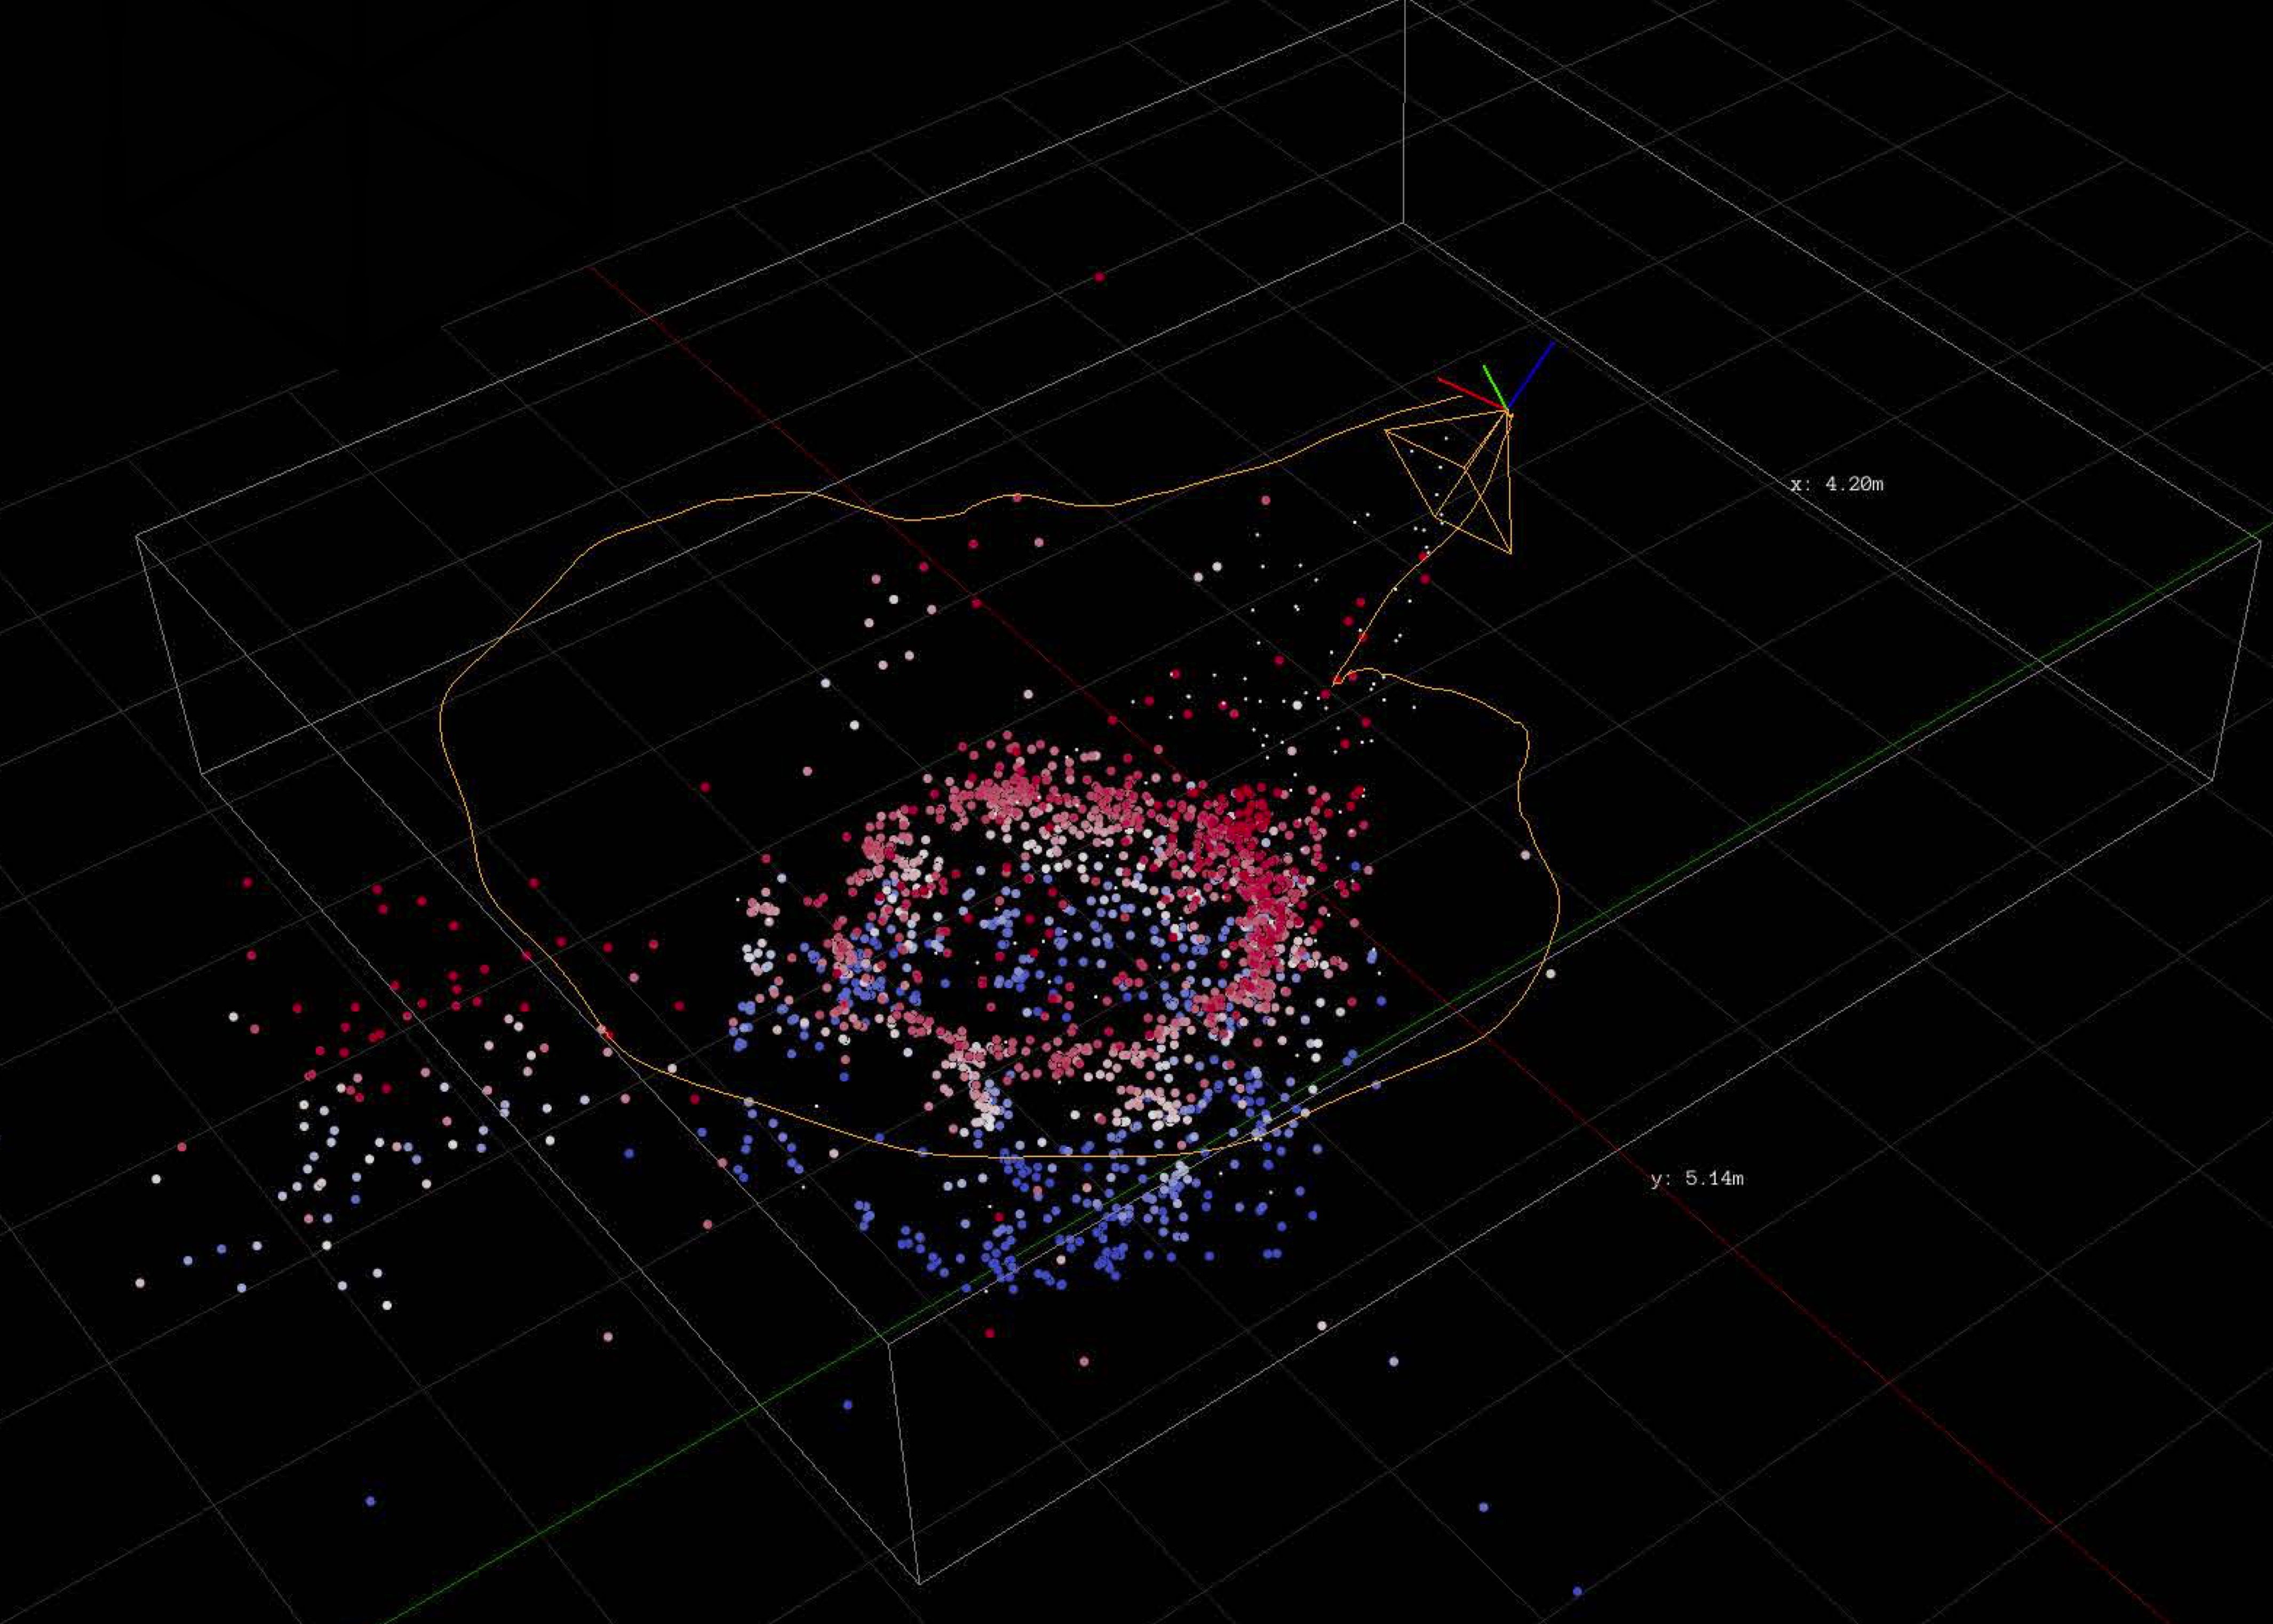
\includegraphics[width=.5\textwidth]{arworldmap-featurepoints}
      \caption{Feature Points}
      \label{FeaturePoints}
    \end{figure}

    In Abbildung \ref{FeaturePoints} ist zu sehen wie so eine Wolke von Feature Points im Raum aussehen kann.

    Der Vorteil dieses Verfahrens ist es, dass keine extenen Geräte oder Marker benötigt werden. Auch ist die Genauigkeit konstant hoch, da nicht nur ein Punkt (Image Marker), sonderen mehrere Punkte (Feature Points) gespeichert werden. Mit moderner Hardware wie LiDAR Sensoren, lässt sich die Performance noch weiter verbessern ohne die Technologie zu ändern.
    Der Nachteil ist, dass die Feature Points nicht abgeglichen werden können, wenn sich der Raum ändert, wenn also Gegenstände oder Möbel dem Raum hinzugefügt werden oder entfernt werden.
    Auch kann es bei großen Räumen zu einer großen Datenmenge kommen, wenn viele Feature Points extrahiert werden.

    \paragraph{Unsere Umsetzung}

    Bei der Auswahl des Verfahrens mussten wir zwischen \textit{Image Marker} und \textit{Visual Positioning System} abwägen.
    Wir haben uns für das \textit{Visual Positioning System} entschieden, da wir dadurch konstant gutes Tracking garantieren können und
    gleichzeitig durch den Einsatz von LiDAR-Technologie auch sehr schnell Szenen speichern und erkennen können.

    Da wir für die Platform iOS entwickeln, nutzen wir die \textit{ARWorlMap} API \footnote{https://developer.apple.com/documentation/arkit/arworldmap}.
    Wenn der Kurator Modus der App gestartet wird, werden automatisch Feature Points gesammelt.
    Wenn der Kurator nun ein Asset im Raum platziert, wird ein sogeannten \textit{ARAnchor} angelegt. Dies ist ein manuell generierter Feature Point.
    In der Dokumentation heißt es: 
    \begin{quote}
      Adding an anchor to the session helps ARKit to optimize world-tracking accuracy in the area around that anchor, so that virtual objects appear to stay in place relative to the real world. If a virtual object moves, remove the corresponding anchor from the old position and add one at the new position.
    \end{quote}
    Dies bedeutet, dass wir zusätzlich zu den automatisch erfassten Feature Points auch speziell auf bestimmte Bereiche achten können, die uns interessieren.
    Wir wollen, dass da wo der Kurator die Assets platziert, besonders genau auf die Position geachtet wird, damit es keine Verschiebungen der Positionen gibt.
    Durch den Einsatz von \textit{ARAnchor} ist dieses gesichert.

    Nachdem der Kurator die Szene fertig bearbeitet hat, wird ein Datensatz erstellt, der alle Anchor und Feature Points enthält.
    Dieser Datensatz wird auf unseren Server hochgeladen und in der Datenbank hinterlegt.

    Wenn nun ein Besucher die App nutzt, werden die Daten auf das entsprechende Gerät geladen.
    Durch Bewegen im Raum werden Feuture Points erkannt. Wenn genügend Punkte gefunden wurden, können diese mit den Punkten aus dem Datensatz abgeglichen werden und somit die genaue Position aller Assets wiederhergestellt werden.


    \begin{figure}[h]
      \centering
      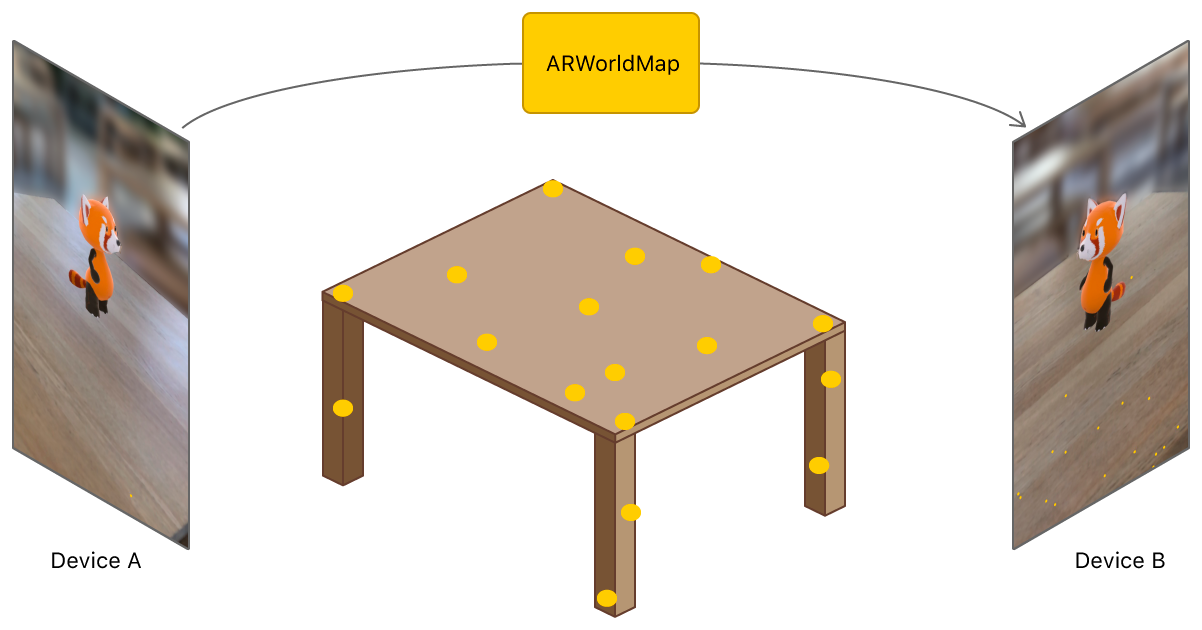
\includegraphics[width=.5\textwidth]{ar-world-map}
      \caption{ARWorldMap Synchronisierung}
      \label{ARWorldMap}
    \end{figure}

    In Abbildung \ref{ARWorldMap} ist zu sehen, wie anhand von Feature Points (gelb) die AR Session synchronisiert wird.

  \section{Wissenschaftliche Umsetzung}
  % Inwiefern wurde hier wissenschaftlich gearbeitet? Welche Forschungsfrage/n wurden geklärt und warum sind diese relevant für das Projekt?
  Für die Umsetzung des Projektes wurde die im neuen Ipad Pro erstmalig verbaute LidAR-Technologie verwendet, welche, wie bereits oben beschrieben, die Erkennung von Oberflächen und somit die Platzierung von Objekten in AR verbessert. Um herauszufinden ob die LidAR-Technologie die Immersionstiefe bei AR-Anwendungen erhöht wurden in einem User Research zehn Studenten der Hochschule Fresenius beobachtet und befragt. Die folgenden Kapitel stellen den Forschungsprozess und die Ergebnisse des User Research dar.
  \subsection{Hypothese}
    % Welche Forschungsfrage wurde gewählt und warum?
    Die von uns aufgrund der Forschungsfrage aufgestellte Hypothese lautet demnach folgendermaßen:\\

    \glqq Nutzer die eine virtuelle AR-Szene mit einem Gerät mit LiDAR-Technologie betrachten haben eine bessere User Experience als Nutzer ohne LiDAR. \grqq{}

  \subsection{User Research}
    % Beschreibung des durchgeführten User Research
    Für die Untersuchungen wurden die zehn Studenten der Hochschule Fresenius in zwei Gruppen aufgeteilt. 
    Jede Gruppe sollte die App selbstständig mit einem von uns mitgebrachten Ipad testen. 
    Dabei verfügte eins der Ipads über LiDAR-Technologie und das andere nicht. 
    Nachdem jeder Student die App selbstständig getestet hatte, wurden die Studenten gebeten jeweils zwei Fragebögen auszufüllen. 
    Einen System Usability Scale (SUS) \cite{SUS} Fragebogen und einen AttrakDiff \cite{AttrakDiff} Fragebogen.\\ 
    Der Fragebogen zur System Usability enthält zehn Fragen um die Bedienbarkeit der App zu messen. 
    Nutzer können bei jeder Frage zwischen \glqq Ich stimme zu\grqq, \glqq Ich stimme nicht zu\grqq{} und drei Zwischenschritten wählen.\\ 
    Der AttrakDiff Fragebogen misst die Bedienbarkeit und das Aussehen der App. 
    Der Nutzer muss die App dabei anhand von 28 gegensätzlichen Adjektiv-Paaren bewerten und das zu der App passendere Adjektiv oder einen Zwischenwert der Adjektiv-Paare wählen.

    \subsubsection{Ergebnisse}
      \textbf{System Usability Scale}\\

      %\begin{figure}
      %\centering
      %\begin{subfigure}{.6\textwidth}
      %  \centering
      %  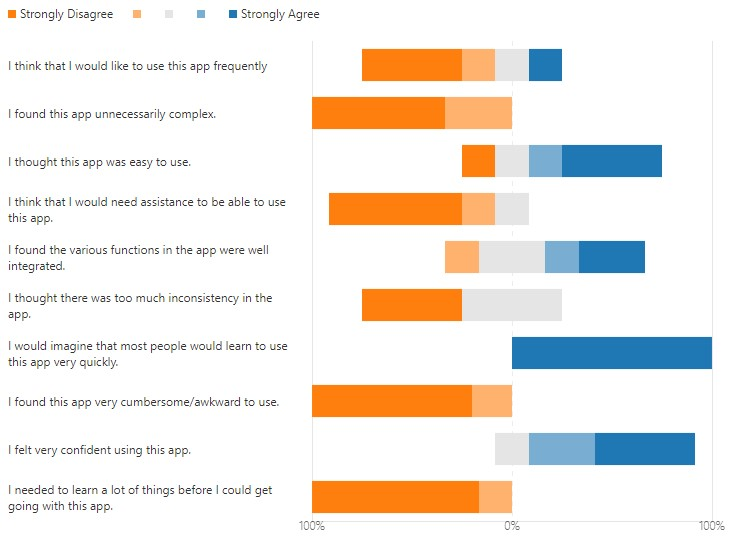
\includegraphics[width=.9\linewidth]{SUS_LiDAR}
      %  \caption{Ergebnisse mit LiDAR}
      %  \label{SUS_L}
      %\end{subfigure}%
      %\begin{subfigure}{.4\textwidth}
      %  \centering
      %  \includegraphics[width=.9\linewidth]{SUS_No_LiDAR_KF_LI}
      %  \caption{Ergebnisse ohne LiDAR}
      %  \label{SUS_NL}
      %\end{subfigure}
      %\caption{SUS Fragebogenergebnisse}
      %\label{fig:test}
      %\end{figure}

      \begin{figure}[h]
      \centering
      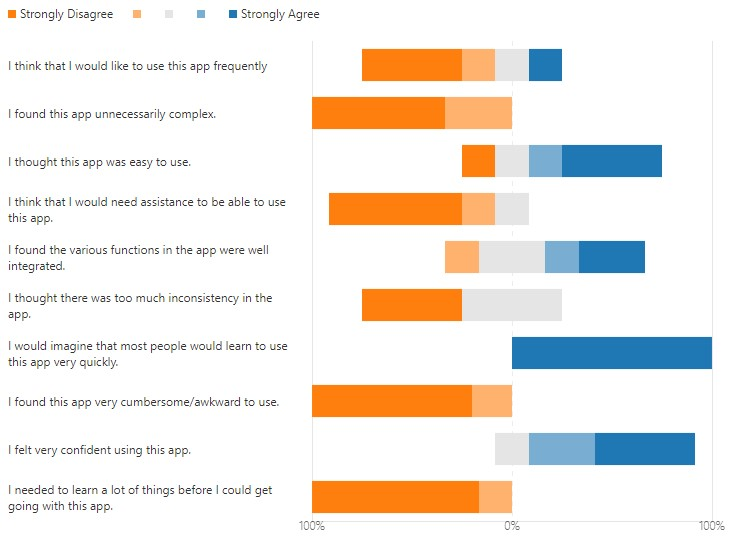
\includegraphics[width=.6\textwidth]{SUS_LiDAR}
      \caption{Ergebnisse des SUS bei Nutzern mit LiDAR}
      \label{SUS_L}
      \end{figure}

      \begin{figure}[h!]
      \centering
      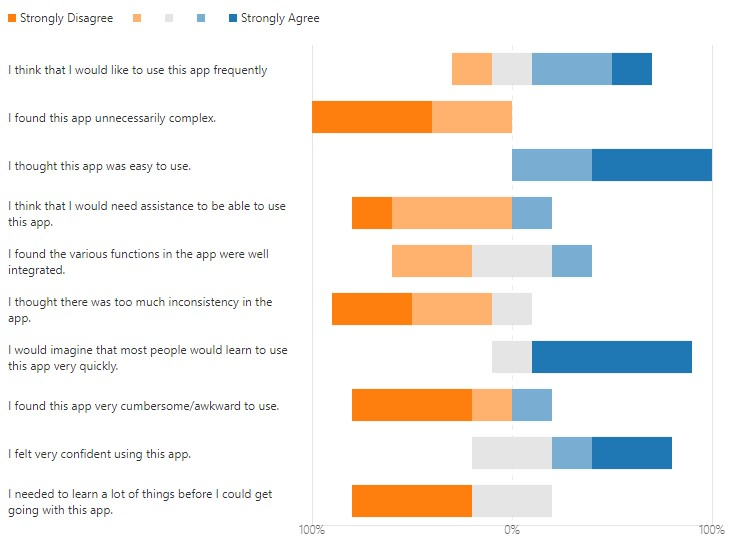
\includegraphics[width=.6\textwidth]{SUS_No_LiDAR}
      \caption{Ergebnisse des SUS bei Nutzern ohne LiDAR}
      \label{SUS_NL}
      \end{figure}

      Wie in Abbildung \ref{SUS_L} und Abbildung \ref{SUS_NL} zu sehen ähneln sich die Ergebnisse des SUS mit und ohne LiDAR Scanner sehr. 
      Die Nutzer fanden die App sowohl mit als auch ohne LiDAR Scanner unkompliziert, leicht erlernbar, wie auch einfach und konsistent in der Benutzung. 
      Einzig bei den Fragen ob die Nutzer die App regelmäßig nutzen würden und ob die Funktionen gut integriert seien gibt es unterschiedliche Meinungen. 
      Die Gruppe ohne LiDAR gab an dass die Funktionen der App weniger gut integriert wären, würden die App allerdings gerne regelmäßig nutzen. 
      Bei der Gruppe mit LiDAR Scanner gaben die Nutzer an die App nicht regelmäßig nutzen zu wollen, fanden die Funktionen der App aber gut integriert.\\

      Eine Auswertung der Fragebögen nach \cite{SUS_Score} ergab einen Wert von 79,5 für die App mit LiDAR Scanner und einen Wert von 75 ohne LiDAR Scanner. 
      Damit erreicht die App sowohl mit als auch ohne LiDAR Scanner ein überdurchschnittliches Ergebnis nach \cite{SUS_Score}.\\

      \textbf{AttrakDiff}\\

      \begin{figure}
      \centering
      \begin{subfigure}{.5\textwidth}
        \centering
        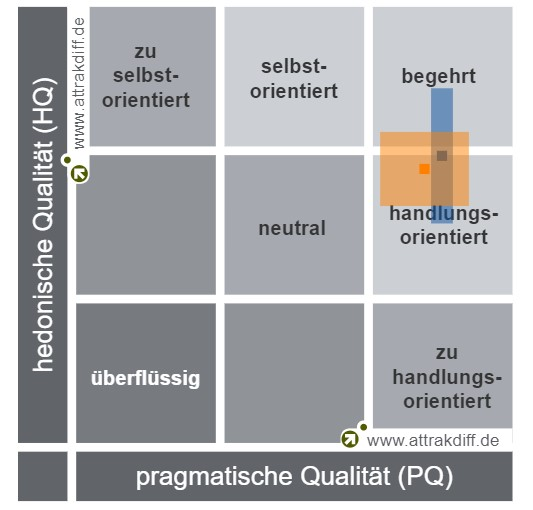
\includegraphics[width=.9\linewidth]{AttrakDiff_Portfolio}
        \caption{Portfolio der AttrakDiff Fragebogenergebnisse}
        \label{AttrakDiff_P}
      \end{subfigure}%

      \begin{subfigure}{.5\textwidth}
        \centering
        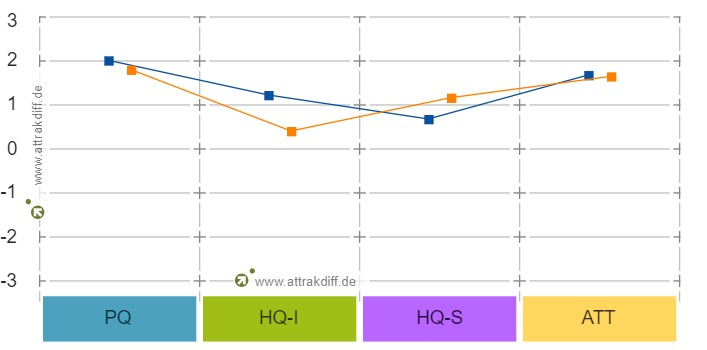
\includegraphics[width=.9\linewidth]{AttrakDiff_Mittelwerte}
        \caption{Mittelwerte der AttrakDiff Fragebogenergebnisse}
        \label{AttrakDiff_M}
      \end{subfigure}

      \caption{AttrakDiff Fragebogenergebnisse; blau: mit LiDAR; orange: ohne LiDAR}
      \label{AttrakDiff}
      \end{figure}

      Die Ergebnisse des AttrakDiff Fragebogens sind in Abbildung \ref{AttrakDiff} und Abbildung \ref{AttrakDiff_WP} zu sehen. 
      Die Fragebogenergebnisse der Gruppe mit LiDAR und ohne LiDAR wurden dabei direkt miteinander verglichen und werden in den Grafiken farblich wie folgt dargestellt: 
      Blau symbolisiert die Ergebnisse des Fragebogens mit LiDAR während Orange die Ergebnisse ohne LiDAR darstellt.\\
      In Abbildung \ref{AttrakDiff_P} sind die aufgestellten Portfolios der beiden Gruppen hinsichtlich hedonischer und pragmatischer Qualität zu sehen. 
      Ein Produkt besitzt pragmatische Qualität, wenn es die Aufgabenlösung effektiv und effizient unterstützt und beziehen sich damit auf Usability im eigentlichen Sinne. 
      Hedonische Qualität geht über die reine Nützlichkeit hinaus und beschreibt Aspekte die dem Nutzer Freude und Spaß bereiten sollen. 
      Das Portfolio spiegelt die Angaben der Nutzer hinsichtlich der pragmatischen und hedonischen Qualität wieder. 
      Je weiter oben im Portfolio das Produkt angeordnet ist, desto besser ist die hedonische Qualität und damit die Freude der Nutzer am Produkt. 
      Eine Einordnung des Produktes im rechten Drittel dagegen zeugt von einem Produkt mit welchem sich die Aufgaben effizient und effektiv lösen lassen. 
      Die Angaben der Nutzer werden in Form eines Rechtecks dargestellt. Je größer das Rechteck ist, desto unsicherer sind sich die Nutzer bezüglich der pragmatischen oder hedonischen Qualität. \\ 
      Sowohl mit als auch ohne LiDAR wurde die App als \glqq handlungsorientiert\grqq{} eingestuft, wobei die Unsicherheit bei der Gruppe ohne LiDAR hier größer ist.\\
      In Abbildung \ref{AttrakDiff_M} werden die Ergebnisse bezüglich der hedonischen Qualität weiter in Stimulation und Identität aufgeschlüsselt. 
      Hedonische Identität bezieht sich dabei auf die Möglichkeit seine Identität durch das Produkt ausdrücken zu können und sich mit dem Produkt selber und seinem Image zu identifizieren. 
      Die Dimension der Stimulation bildet ab, inwieweit das Produkt das Bedürfnis sich weiterzuentwickeln unterstützt, indem es neuartige, interessante und anregende Funktionalitäten, Inhalte, Interaktions- und Präsentationsstile bietet. 
      Abbildung \ref{AttrakDiff_M} bestätigt, dass die pragmatische Qualität sowohl mit als auch ohne LiDAR mit einem Wert von ungefähr 2 überdurchschnittlich ist. Auch die Attraktivität des Produktes wird überdurchschnittlich hoch eingeschätzt. Die hedonischen Qualitäten der Identität und Stimulation sind dagegen mit einem Wert von ca. 1 eher durchschnittlich.\\
      Abbildung \ref{AttrakDiff_WP} zeigt die mittleren Ausprägungen der einzelnen Wortpaare des AttrakDiff Fragebogens. 
      Die mittleren Ausprägungen der Wortpaare sind sowohl mit als auch ohne LiDAR sehr ähnlich. Die App wurde beide Male als einfach zu handhaben, direkt und handhabbar bewertet. 
      Außerdem wurde die App mit dem LiDAR Scanner als sehr einbeziehend und vorzeigbar eingeschätzt. Bei der App ohne LiDAR sind diese Eigenschaften nicht so stark ausgeprägt.\\
      Ein Unterschied besteht beim herkömmlich-neuartig Adjektiv-Paar. Die App ohne LiDAR wurde als sehr neuartig eingeschätzt, während die App mit LiDAR als herkömmlich bewertet wurde.
      Abschließend wurde die App mit LiDAR als äußerst gut bewertet, ohne LiDAR fiel die Wertung etwas schlechter aus.\\
  
      \begin{figure}[h!]
      \centering
      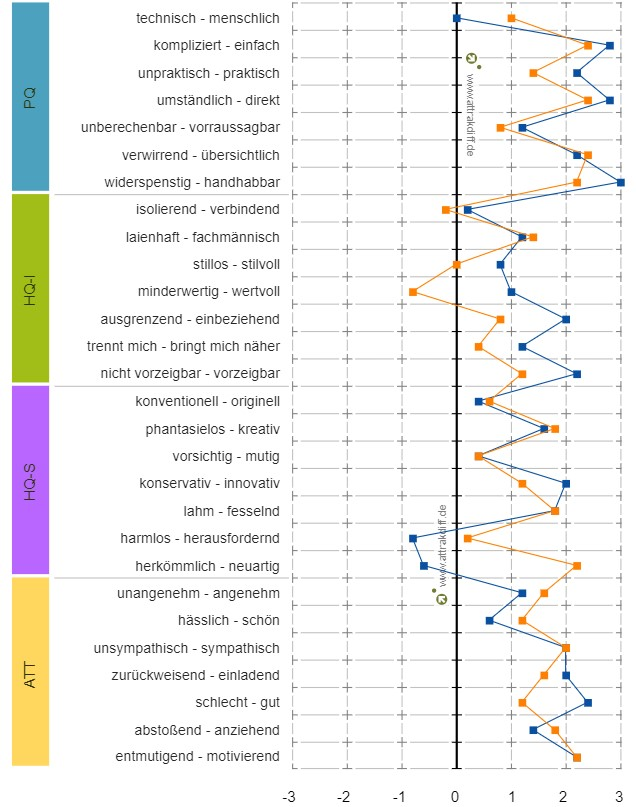
\includegraphics[width=.6\textwidth]{AttrakDiff_Wortpaare}
      \caption{AttrakDiff Wortpaare; blau: mit LiDAR; orange: ohne LiDAR}
      \label{AttrakDiff_WP}
      \end{figure}

      \subsection{Analyse der Ergebnisse}
        % Analyse der während des User Research gesammelten Daten
        Anhand der Fragebogendaten kann die Hypothese, dass LiDAR die User Experience und Immersion verbessert, nicht eindeutig bestätigt werden. Die Ergebnisse der SUS Fragebögen waren sich sehr ähnlich und auch beim AttrakDiff Fragebogen gibt es nur geringe Unterschiede. Aufgrund der Ergebnisse des AttrakDiff Fragebogens wurde die App mit LiDAR Unterstützung als ein wenig besser implementiert und vorzeigbar bewertet, allerdings gaben die Nutzer an die App ohne LiDAR regelmäßiger benutzen zu wollen.\\
        Anhand des geringen Stichprobenumfangs von fünf Personen pro Umfrage fallen individuelle Präferenzen stark ins Gewicht. Für eine aussagekräftigere Studie müssten mehr Versuchsteilnehmer befragt werden.\\

        Obwohl die Ergebnisse der Fragebögen keine stichhaltigen Ergebnisse erbrachten konnten die Aussagen der Versuchsteilnehmer während der Studie für die weitere Entwicklung nützliche Ergebnisse erbringen. Die Versuchsteilnehmer teilten uns bspw. mit dass das Scrollen der App-Auswahl nicht intuitiv sei, da die Gesten welche normalerweise auf mobilen Touchgeräten zum Scrollen verwendet werden nicht unterstützt wurden. Statt der normalen \glqq Swipe\grqq -Geste musste mit einer Scroll-Leiste an der Seite der UI gescrollt werden. Weiterhin fanden die Nutzer die Startseite der App verwirrend, da die Buttons zum Betreten der Szene als Besucher und Kurator schlecht als solche ausgezeichnet waren und einige Nutzer nicht wussten was sie tun konnten um die App zu benutzen. Eine weitere Funktionalität welche von den Nutzern erwartet wurde war das Positionieren, Rotieren und Skalieren von bereits platzierten Modellen. Die Nutzer verwendeten automatisch die hierfür erlernten Gesten und waren verwirrt und enttäuscht wenn sie feststellen mussten, dass diese keinerlei Auswirkungen haben.\\

        Neben Funktionalitäten der App welche fehlten oder noch nicht gut genug implementiert waren, teilten uns mehrere Nutzer mit, dass die App \glqq einfach zu benutzen\grqq{} und die Kern-Funktionen der App, das Auswählen und Platzieren von Modellen intuitiv verständlich sei.
        \section{Schlussfolgerungen}
        % Wie können die bei der Analyse gewonnenen Ergebnisse in das Projekt integriert werden? Bzw. wie wurden die Ergebnisse bereits integriert?
        Anhand der Ergebnisse der Fragebögen und der Auswertung der Beobachtungen der Nutzer beim Verwenden der App, sowie deren Kommentare, implementierten wir einige Änderungen am User Interface und integrierten neue, intuitiv von den Nutzern erwartete, Funktionen.\\
        Wir passten das User Interface in zweierlei Hinsicht an. Als Erstes änderten wir den Startbildschirm der App, um den Nutzern einen einfacheren Einstieg zu ermöglichen. Anstatt als Erstes den Modus, sprich Besucher oder Kurator, wählen zu müssen, wird der Nutzer nun aufgefordert einen Marker zu Scannen und kann daraufhin auswählen in welchem Modus er die Szene betritt.\\
        Um die Erwartungen der Nutzer in der App zu bedienen, änderten wir das Scroll-Verhalten der Asset-Auswahl, sodass die Nutzer wie gewohnt mit Gesten die Liste scrollen können. In diesem Zuge implementierten wir ebenfalls die von den Nutzern gewünschten Funktionen bereits platzierte Modelle später neu zu positionieren, rotieren und skalieren. Diese Funktionen wurden ebenfalls mit den von mobilen Geräten bereits bekannten Gesten implementiert.\\

        Durch die Kommentare der Nutzer und den Beobachtungen während der Nutzung konnten wir das User Interface der App deutlich verbessern und so die Nutzerzufriedenheit steigern. Die überarbeitete Version der App wurde bei späteren Demonstrationen intuitiver und besser angenommen.
        
      \section{Ausblick}
        % Wie könnte das Projekt in Zukunft erweitert werden?
        % PDF Unterstützung / PDFs in AR
        % AI-basierter Vorschlag ähnlicher Inhalte zum schnellen Platzieren (Quick Placement)
        % Erstellen von Lichtquellen in der AR Szene und Export der Lichtquellen als GLTF
        % Schatten
        % Integration von externen APIs wie Sketchfab oder Google Poly
        % Tutorial bei der erstmaligen Benutzung der App
        % Weitere Informationen über digitale Inhalte via dynamisch erstellter AR-Textfelder
        % Login-Maske um das Platzieren von Inhalten als Kurator zu schützen
        % Szenen direkt in der App neu erstellen und Namen ändern
        % Bilder und Videos automatisch an Wänden platzieren
        % Angepasstes App-UI für Smartphones
        Auch wenn die App bereits in einem funktionierenden Stadium ist, gibt es immer noch Features die in Zukunft ergänzt werden könnten. 
        Die im Folgenden vorgestellten Ideen stellen eine Auswahl an Features da, welche die Nutzbarkeit der App verbessern und für einen breiteren Markt öffnen.\\
        In der App können bereits Bilder, Videos und 3D-Modelle dargestellt werden. Denkbar wäre weiterhin eine Darstellung von PDFs in AR. 
        So könnten bspw. studentische oder wissenschaftliche Arbeiten ebenfalls virtuell ausgestellt werden.\\
        Auch wenn das Platzieren von Modellen bereits gut funktioniert, so ist die Auswahl mehrerer Modelle mühsam. 
        Für jedes Modell muss das UI geöffnet und das gewollte Modell ausgewählt werden. 
        Eine Verbesserung wäre hier eine durch eine AI unterstützte Schnellauswahl, welche dem User basierend auf dem gerade platzierten Modell thematisch ähnliche Modelle, z.B. aus demselben Studiengang, vorschlägt. 
        So könnte der Workflow des Platzierens in der App erleichtert werden.\\
        Und während bei 3D-Modellen die Platzierung mitten im Raum häufig gewollt ist um das Modell von allen Seiten betrachten zu können, sind in der Luft schwebende Bilder und Videos unter Umständen nicht gewollt. 
        Aus diesem Grund sollten zwei-dimensionale Objekte wie Bilder oder Videos automatisch an physikalischen Entitäten wie Wänden platziert werden, sodass der Eindruck entsteht die Medien würden wie in einem Museum an den Wänden hängen.\\
        Auch das Platzieren von Lichtquellen in der Szene ist geplant, um die Lichtverhältnisse in AR den Lichtverhältnissen der Realität besser anzupassen oder Highlights auf bestimmte Inhalte zu setzen. 
        Dazu müssen Lichtquellen in AR über das App-Interface platzierbar gemacht und beim Speichern der Szene in der Datenbank gespeichert werden.\\
        Zusammen mit der Implementierung von virtuellen Lichtquellen läge die Einführung von Schatten, welche die Modelle in AR werfen, nahe. 
        Lichtquellen und Schatten würden die virtuellen Ausstellungen noch lebendiger und realer werden lassen.\\
        Um den Informationsgehalt der virtuellen Ausstellungen zu erhöhen ist die Darstellung der Künstlerdaten, wie Name des Künstlers, Name des Modells, etc. geplant. 
        In einem Text-UI sollen diese, bereits in der Datenbank vorliegenden, Daten dynamisch erstellt und dargestellt werden.\\
        Für die HAW Hamburg ist die Anbindung an eine, von den Studenten der HAW genutzten, Datenbank zwar sinnvoll, für andere interessierte Institutionen wie andere Hochschulen oder Museen allerdings weniger. 
        Aus diesem Grund planen wir die Anbindung der APP an externe APIs wie Sketchfab und Google Poly, wo jeder 3D-Modelle hochladen und nutzbar machen kann. So ist die App nicht mehr nur von unserer selbst entworfenen Datenbank abhängig, sondern kann automatisch auf große Modell-Bibliotheken zugreifen.\\
        Damit von Kuratoren erstellte virtuelle Szenen nicht von Außenstehenden frei verändert werden können ist die Implementierung einer Login-Maske als Kurator in der Diskussion.\\
        Und um die Handhabung der App und das Erstellen von Szenen weiter zu vereinfachen gibt es Pläne neue Szenen direkt in der App erstellen zu können. Zur Zeit können diese ausschließlich über ein Interface auf dem CMS erstellt werden. 
        Um diesen Schritt zu umgehen und nicht mehr von einer zweiten Application abhängig zu sein könnte dieser erste Schritt bereits in der App passieren. Weiterhin sollte der Szenen-Name direkt über die App und nicht nur über das Content-Management-System änderbar sein.\\
        Die letzten beiden Ideen handeln von einem Tutorial für Erstnutzer, welches die Funktionen der App anschaulich beim Ersten Öffnen zeigt und die Erfahrung des Nutzers so verbessert und einem angepassten Interface für Smartphones. 
        Das jetzige Interface der App ist für das neue Ipad Pro mit LiDAR-Scanner optimiert und funktioniert bei bspw. dem neuen Iphone 12 Pro nicht optimal. Eine Anpassung des User Interfaces an unterschiedliche Gerätetypen wäre bei einer wachsenden Auswahl an unterstützten Geräten wünschenswert.\\

        Wie zu sehen ist, ist das Potenzial der App bei Weitem noch nicht ausgeschöpft und wird auch in Zukunft von uns weiter entwickelt und verbessert werden. 
        Die hier vorgestellten Features stellen unsere Ideen für eine mögliche zukünftige Erweiterung der App dar.

  \bibliography{literature}        
  \bibliographystyle{IEEEtran}

\end{document}
